% arara: xelatex
% arara: xelatex
% arara: xelatex

% options:
% thesis=B bachelor's thesis
% thesis=M master's thesis
% czech thesis in Czech language
% english thesis in English language
% hidelinks remove colour boxes around hyperlinks

\documentclass[thesis=M,english]{FITthesis}[2019/12/23]

\usepackage[utf8]{inputenc} % LaTeX source encoded as UTF-8

\usepackage{graphicx} %graphics files inclusion
\usepackage{amsmath} %advanced maths
\usepackage{amssymb} %additional math symbols 
\usepackage{mathtools,amscd}

\usepackage{dirtree} %directory tree visualisation
\usepackage{listings}
\usepackage{pdfpages}
\usepackage{float}
\usepackage{svg}

\usepackage{mmacells}
\mmaSet{leftmargin=2em}

% % list of acronyms
% \usepackage[acronym,nonumberlist,toc,numberedsection=autolabel]{glossaries}
% \iflanguage{czech}{\renewcommand*{\acronymname}{Seznam pou{\v z}it{\' y}ch zkratek}}{}
% \makeglossaries

% % % % % % % % % % % % % % % % % % % % % % % % % % % % % % 
% EDIT THIS
% % % % % % % % % % % % % % % % % % % % % % % % % % % % % % 

\department{Department of Information Security}
\title{Multivariate cryptography}
\authorGN{Jan} %author's given name/names
\authorFN{Rahm} %author's surname
\author{Jan Rahm} %author's name without academic degrees
\authorWithDegrees{Bc. Jan Rahm} %author's name with academic degrees
\supervisor{Ing. Jiří Buček, Ph.D.}
\acknowledgements{I would like to thank Ing. Jiří Buček, Ph.D. for the willingness, consultation and valuable advice he gave me.}
\abstractEN{The diploma thesis deals with selected algorithms of multivariate cryptography, especially Unbalanced Oil \& Vintage and Rainbow. The aim of this work is implementation of algorithms in Wolfram Mathematica, investigation of existing solutions and their implementation on ESP32 microcontroller. The algorithms are tested and measured against the RSA and ECDSA algorithms.}
\abstractCS{Diplomová práce se zabývá vybranými algoritmy multivariační kryptografie, zejména Unbalanced Oil \& Vintage a Rainbow. Cílem práce je implementace algoritmů ve Wolfram Mathematica, prozkoumání již existujících řešeních a jejich implementace na mikrokontroleru ESP32. Algoritmy jsou otestovány a změřeny vůči algoritmům RSA a ECDSA.}
\placeForDeclarationOfAuthenticity{Prague}
\keywordsCS{Multivariační kryptografie, Unbalanced Oil \& Vintage, Rainbow, Wolfram Mathematica, ESP32}
\keywordsEN{Multivariate cryptography, Unbalanced Oil \& Vintage, Rainbow, Wolfram Mathematica, ESP32}
\declarationOfAuthenticityOption{1} %select as appropriate, according to the desired license (integer 1-6)
\website{https://github.com/rahmjan/Diploma_Thesis} %optional thesis URL

\begin{document}

% \newacronym{CVUT}{{\v C}VUT}{{\v C}esk{\' e} vysok{\' e} u{\v c}en{\' i} technick{\' e} v Praze}
% \newacronym{FIT}{FIT}{Fakulta informa{\v c}n{\' i}ch technologi{\' i}}

%%%%%%%%%%%%%%%%%%%%%%%%%%%%%%%%%%%%%%%%%%%%
%%%%%%%%%%%%%%%%%%%%%%%%%%%%%%%%%%%%%%%%%%%%
\setsecnumdepth{part}
\chapter{Introduction}
Cryptography is one of the most needed part of modern informatics because almost everyone has something they wish to stay private. But today we can see uprise of the quantum computers which are able to decipher the conventional algorithms for cryptology. That is why a new category of post-quantum cryptography was created and one of its candidates is multivariate cryptography.

The objective of this work is to describe principles of multivariate cryptography for educational purpose with creation of simple example in Wolfram Mathematica. The focus is on Unbalanced Oil \& Vintage and Rainbow algorithms with examination of reference implementation. Further focusing on possible implementation on ESP32 and possible use in IoT.

The final part belongs to comparison with conventional algorithms which are RSA and ECDSA.

%%%%%%%%%%%%%%%%%%%%%%%%%%%%%%%%%%%%%%%%%%%%
%%%%%%%%%%%%%%%%%%%%%%%%%%%%%%%%%%%%%%%%%%%%
\setsecnumdepth{all}
\chapter{Basic terms and definitions}
The chapter describes concepts and algorithms used in the thesis.

\section{Basic terms}
\subsection{Polynomial}
Polynomial $p$ is function to which applies
\[
	p(x) = \sum\limits_{i=0}^n {\alpha_ix^i} = \alpha_0 + \alpha_1x + \alpha_2x^2 + ... + \alpha_nx^n,
\]
where $n \in N_0$ and $\alpha_0, \alpha_1, ..., \alpha_n \in R$. Values $\alpha_0, \alpha_1, ..., \alpha_n$ we calls polynomial coefficients of $p$.  

\subsection{Degree of a polynomial}
The degree of a polynomial is the highest index $i \in N_0$ to which applies that coefficient $\alpha_i \ne 0$. If all coefficients are zero, then the degree of the polynomial is -1.

\subsection{Post-quantum cryptography}
It refers to algorithms that are thought to be secure against an attack by a quantum computer.

But today it is not true for the most used cryptographic algorithms, which are based on mathematical problems of integer factorization, discrete logarithm or elliptic-curve discrete logarithm. These problems can be solved by Shor's algorithm on quantum computer.

\subsection{Finite field}
A finite field is a finite set which is a field. This means that multiplication, addition, subtraction and division (excluding division by zero) are defined and satisfy the rules of arithmetic known as the field axioms.

The simplest examples of finite fields are the fields of prime order: $\mathbb {F}_{p}$ may be constructed as the integers modulo p.

\subsection{Translation}
In Euclidean geometry, a translation is a geometric transformation that moves every point of a figure or a space by the same distance in a given direction.

\subsection{Linear map}
In mathematics, a linear map is a mapping $V \rightarrow W$ between two modules (for example, two vector spaces) that preserves the operations of addition and scalar multiplication.

\subsection{Affine map}
An affine map is the composition of two functions: a translation and a linear map. Ordinary vector algebra uses matrix multiplication to represent linear maps, and vector addition to represent translations. Formally, in the finite-dimensional case, if the linear map is represented as a multiplication by a matrix $A$ and the translation as the addition of a vector $\vec {b}$, an affine map $f$ acting on a vector ${\vec {x}}$ can be represented as:
\[
{\vec {y}}=f({\vec {x}})=A{\vec {x}}+{\vec {b}}
\]

\subsection{Wolfram Mathematica}
Wolfram Mathematica is a computer program widely used in scientific, technical and mathematical circles. The program was originally created by Stephen Wolfram and further developed by a team of mathematicians and programmers. It is sold by Wolfram Research, with headquartered in Champaign, Illinois.

\subsection{IoT}
Internet of Things (IoT) is a term in computer science for a network of physical devices, vehicles, household appliances, or other devices that are equipped with electronics, software, sensors, moving parts, or network connectivity that allows these devices to connect and exchange data.

\subsection{Valgrind}
Valgrind is a computer program for Unix systems that helps in debugging and profiling programs. For example, it can be used to search for memory leaks, concurrencies, or to monitor cache usage. Valgrind is open source software distributed under the GPL license.

\subsection{PRNG}
The pseudo-random number generator (PRNG) is a deterministic program that generates a sequence of numbers. If using statistical tests the sequence should be indistinguishable from random as much as possible.

\subsection{ESP32}
The ESP32 is a low-cost, low-power microcontroller with integrated Wi-Fi and Bluetooth. It is created and developed by Espressif Systems, a Chinese company based in Shanghai, and is manufactured by TSMC using a 40 nm process.

\bigskip
\noindent
Basic technical parameters are:
\begin{itemize}
\item	CPU: Xtensa dual-core
\item	Memory: 520 KiB SRAM
\item	Wi-Fi: 802.11 b/g/n
\item	Bluetooth: v4.2 BR/EDR and BLE
\item	IEEE 802.11 standard
\item	Hardware acceleration: AES, SHA-2, RSA, ECC, RNG
\end{itemize}

\subsection{RSA}
RSA is algorithm for cryptographic and signature scheme. Name comes from initials of authors Rivest, Shamir and Adleman.

\bigskip
\noindent
RSA security is based on the problem of factorization, an assumption that breaking a large number into a product of prime numbers is a difficult task. From the number $n = pq$ it should be almost impossible to determine the factors $p$ and $q$ in a reasonable time, because there is no known factorization algorithm working in polynomial time to the size of the binary notation of $n$. On the other side, multiplying two large numbers is very easy.

\subsection{ECDSA}
Elliptic curve digital signature protocol (ECDSA) is a variant of the DSA protocol that uses elliptic curves for digital signatures.

\bigskip
\noindent
The security of elliptic curve is based on the problem of discrete logarithm where is an assumption that finding $k$ of $Y \equiv g^k (mod \, p)$ is a difficult task.

%%%%%%%%%%%%%%%%%%%%%%%%%%%%%%%%%%%%%%%%%%%%
\newpage
\section{Multivariate cryptography}
\subsection{Definition}
"Multivariate cryptography (MC) is the generic term for asymmetric cryptographic primitives based on multivariate polynomials over a finite field $\mathbb{F}$."\cite{L-WIKI1}

It means it is system of nonlinear polynomial equations with coefficients over a finite filed $\mathbb{F} = \mathbb{F}_q$ with $q$ elements:
\[
	p^{(1)}(x_1,\ldots,x_n) = \sum\limits_{i=1}^{n} {\sum\limits_{j=1}^{n} {p_{ij}^{(1)} \cdot x_ix_j}} + \sum\limits_{i=1}^{n} {p_{i}^{(1)} \cdot x_i} + p_0^{(1)}
\]
\[
	p^{(2)}(x_1,\ldots,x_n) = \sum\limits_{i=1}^{n} {\sum\limits_{j=1}^{n} {p_{ij}^{(2)} \cdot x_ix_j}} + \sum\limits_{i=1}^{n} {p_{i}^{(2)} \cdot x_i} + p_0^{(2)}
\]
\[
	\vdots
\]
\[
	p^{(m)}(x_1,\ldots,x_n) = \sum\limits_{i=1}^{n} {\sum\limits_{j=1}^{n} {p_{ij}^{(m)} \cdot x_ix_j}} + \sum\limits_{i=1}^{n} {p_{i}^{(m)} \cdot x_i} + p_0^{(m)}
\]
 
If the polynomials are of degree two, they are called multivariate quadratics (MQ). Solving systems of multivariate polynomial equations is proven to be NP hard, so called MQ Problem. That is the reason why MC is often considered to be good candidate for post-quantum cryptography.

MC is very fast and requires only moderate computational resources, which makes it attractive for applications in low-cost devices.

\subsection{MQ Problem}
Given $m$ quadratic polynomials $p^{(1)}(x),\ldots,p^{(m)}(x)$ in the $n$ variables $x_1,\ldots,x_n$, find a vector $\bar{x} = (\bar{x}_1,\ldots,\bar{x}_n)$ such that $p^{(1)}(\bar{x}) = \ldots = p^{(m)}(\bar{x}) = 0$.

\subsection{Public key}
The public key of MC is system of MC polynomials. To build this system based on MQ Problem, it needs an easily invertible quadratic map $\mathcal{F}: \mathbb{F}^n \rightarrow \mathbb{F}^m$, so called \textit{central map}. Because it is easily invertible, it needs to be hidden in public key by invertible affine maps: $\mathcal{S}: \mathbb{F}^m \rightarrow \mathbb{F}^m$ and $\mathcal{T}: \mathbb{F}^n \rightarrow \mathbb{F}^n$.

The public key of this system is composed map:
\[
	\mathcal{P} = \mathcal{S} \circ \mathcal{F} \circ \mathcal{T} : \mathbb{F}^n \rightarrow \mathbb{F}^m
\]
and the private key consists of the tree maps $\mathcal{S}$, $\mathcal{F}$ and $\mathcal{T}$, also known as \textit{trapdoor}.

Public key should be hard to invert without the knowledge of the \textit{trapdoor}.

\begin{figure}[h]
\begin{equation*}
  \begin{CD}
     z \in \mathbb{F}^n @>  \mathcal{P} >> w \in \mathbb{F}^m \\
    @V\mathcal{T}VV  @A\mathcal{S}AA \\
  y \in \mathbb{F}^n @> \mathcal{F} >> x \in \mathbb{F}^m
  \end{CD}
\end{equation*}
\caption{Workflow of multivariate public key cryptosystems}
\end{figure}
\smallskip

\subsection{Encryption}
To get a ciphertext $w$, message $z \in \mathbb{F}^n$ can by easily encrypted by evaluation of the public key $\mathcal{P}$:
\[
	w = \mathcal{P}(z) \in \mathbb{F}^m
\]
For decryption of ciphertext, it needs to be evaluated by private key in tree steps: 
\[
	x = \mathcal{S}^{-1}(w) \in \mathbb{F}^m, \, y = \mathcal{F}^{-1}(x) \in \mathbb{F}^n, \, z = \mathcal{T}^{-1}(y) \in \mathbb{F}^n
\]
There is a condition that requires to be $m \geq n$, this way the public key $\mathcal{P}$ will be injective and decryption will output a unique plaintext.

\subsection{Signature}
To generate a signature for a message $m$, it needs to use a hash function:
\[
	\mathcal{H}: \{0,1\}^{*} \rightarrow \mathbb{F}^m
\]
to compute the hash value:
\[
	w = \mathcal{H}(m) \in \mathbb{F}^m
\]
After this step it can be evaluated by:
\[
	x = \mathcal{S}^{-1}(w) \in \mathbb{F}^m, \, y = \mathcal{F}^{-1}(x) \in \mathbb{F}^n, \, z = \mathcal{T}^{-1}(y) \in \mathbb{F}^n
\]
where $z$ is the signature of message $m$. As can be seen, it is similar to description of ciphertext.

The verification of signature $z$ is done by computing the hash value:
\[
	w = \mathcal{H}(m) \in \mathbb{F}^m
\]
and by evaluation of public key $\mathcal{P}$:
\[
	w' = \mathcal{P}(z) \in \mathbb{F}^m
\]
If $w' = w$ is true, the signature is valid, otherwise not.

There is also condition that requires to be $m \leq n$, this way the public key $\mathcal{P}$ will be surjective and private key can sign any message.

%%%%%%%%%%%%%%%%%%%%%%%%%%%%%%%%%%%%%%%%%%%%
\section{UOV}
The Unbalanced Oil and Vinegar's name comes from the fact that the variables of the polynomials are grouped into two groups: the vinegar and the oil. These two groups are mixed in the polynomials and the unbalanced attribute refers to the ratio of the variables, where is always more vinegar than oil variables. The signature scheme was proposed by Kipnis and Patarin in 1999.

\subsection{Definition}
Let $\mathbb{F}$ be a finite field, $v,o \in \mathbb{N}$ and $n=v+o$, $V=\{1, \ldots, v\}$, $O=\{v+1, \ldots, n\}$. The variables $x_1, \ldots, x_v$ are Vinegar variables and $x_{v+1}, \ldots, x_n$ are Oil variables. If $v=o$ the scheme is called balanced Oil \& Vinegar (OV), for $v>o$ it is UOV.

\bigskip
\noindent
The \textit{central map} $\mathcal{F}:\mathbb{F}^n \rightarrow \mathbb{F}^o$ consist of $o$ quadratic polynomials $f^{(1)}, \ldots, f^{(o)}$:
\[
	f^{(k)} = \sum\limits_{i=1}^{v} {\sum\limits_{j=1}^{v} {\alpha_{ij}^{(k)} \cdot x_ix_j}} +  \sum\limits_{i=1}^{v} {\sum\limits_{j=v+1}^{n} {\beta_{ij}^{(k)} \cdot x_ix_j}}+ \sum\limits_{i=1}^{n} {\gamma_{i}^{(k)} \cdot x_i} + \delta^{(k)}
\]
where $\alpha_{ij}^{(k)}$, $\beta_{ij}^{(k)}$, $\gamma_{i}^{(k)}$, $\delta^{(k)} \in \mathbb{F}$ and $1 \leq k \leq o$.

\bigskip
\noindent
To hide $\mathcal{F}$ in the public key, it is combined with one invertible affine map $\mathcal{T}: \mathbb{F}^n \rightarrow \mathbb{F}^n$. The public key of the scheme is in the form:
\[
	\mathcal{P} = \mathcal{F} \circ \mathcal{T} : \mathbb{F}^n \rightarrow \mathbb{F}^o
\]
and the private key consist of $\mathcal{F}$ and $\mathcal{T}$. The second affine map $\mathcal{S}$ is not needed for the security of UOV.

\subsection{Security}
For the security of UOV is required $v \geq 2o$ because of the attack of Kipnis and Shamir on balanced OV.\cite{L-KS98} Besides of that, the UOV scheme resisted (for suitable parameter sets) cryptanalysis for over 20 years. Now it is one of the oldest and best studied cryptosystems and is therefore believed to be of high security.

The UOV scheme is very simple, has small signatures and is fast. The main disadvantage is its public keys which are quite large.

%%%%%%%%%%%%%%%%%%%%%%%%%%%%%%%%%%%%%%%%%%%%
\newpage
\section{Rainbow}
The Rainbow is a multi-layer version of UOV. The layers are not independent from each other but there is a hierarchy which uses the results from the layer above to compute additional variables. The name comes from the link to the layers of a rainbow and the scheme was introduced by Ding and Schmid in 2005.

The main advantage compared to UOV should be in better performance, smaller key sizes and smaller signatures.

\subsection{Definition}
Let $\mathbb{F}$ be a finite field, $0<v_1<v_2<\ldots<v_{u+1} = n$ be a sequence of integers and $V_i=\{1, \ldots, v_i\}$, $O_i=\{v_i+1, \ldots, v_{i+1}\}$ and $o_i = v_{i+1} - v_i \,\, (i=1,\ldots,u)$ where $o_i$ is number of oil variables and $u$ is number of UOV instances.

\bigskip
\noindent
The \textit{central map} $\mathcal{F}:\mathbb{F}^n \rightarrow \mathbb{F}^m$ consist of $m = n - v_1$ quadratic polynomials $f^{(v_1+1)}, \ldots, f^{(n)}$:
\[
	f^{(k)} = \sum\limits_{i,j \in V_l}{\alpha_{ij}^{(k)} \cdot x_ix_j} +  \sum\limits_{i \in V_l,j \in O_l}{\beta_{ij}^{(k)} \cdot x_ix_j}+ \sum\limits_{i \in V_l \cup O_l}{\gamma_{i}^{(k)} \cdot x_i} + \delta^{(k)}
\]
where $l \in \{1, \ldots, u\}$ is the only integer such that $k \in O_l$ and $\alpha_{ij}^{(k)}$, $\beta_{ij}^{(k)}$, $\gamma_{i}^{(k)}$, $\delta^{(k)} \in \mathbb{F}$.

\bigskip
\noindent
To hide $\mathcal{F}$ in the public key, it is combined with two invertible affine maps $\mathcal{T}: \mathbb{F}^n \rightarrow \mathbb{F}^n$ and $\mathcal{S}: \mathbb{F}^m \rightarrow \mathbb{F}^m$. The public key of the scheme is in the form:
\[
	\mathcal{P} = \mathcal{S} \circ \mathcal{F} \circ \mathcal{T} : \mathbb{F}^n \rightarrow \mathbb{F}^m
\]
and the private key consist of $\mathcal{S}$, $\mathcal{F}$ and $\mathcal{T}$.

%%%%%%%%%%%%%%%%%%%%%%%%%%%%%%%%%%%%%%%%%%%%
%%%%%%%%%%%%%%%%%%%%%%%%%%%%%%%%%%%%%%%%%%%%
\chapter{Realization}
Chapter describes implementation of algorithms on selected platforms which are Wolfram Mathematica, PC and microcontroller ESP32. For the last two specified the implementation is in language C++.

\section{Wolfram Mathematica}
This section describes examples in Wolfram Mathematica and step by step description of algorithms.

\subsection{UOV}
Here is description of signature scheme of UOV. This example of UOV is in fact example of balanced OV because it simplify the explanation of the algorithm.

\bigskip
\noindent
First set up the parameters of the example: 
Let $\mathbb{F} = GF(7)$, $o=v=3$. The central map $\mathcal{F} = (f^{(1)}, f^{(2)}, f^{(3)})$ is given by:
\begin{mmaCell}[addtoindex=2,moredefined={mod, F1, F2, F3},morepattern={x1_, x2_, x3_, x4_, x5_, x6_, x1, x2, x3, x4, x5, x6}]{Input}
  mod=7;
  F1[x1_,x2_,x3_,x4_,x5_,x6_]:=
4x1^2+4x1*x3+5x1*x4+6x1*x5+x1*x6+6x1+4x2^2+x2*x3+6x2*x4
+6x2*x5+5x2*x6+5x2+5x3^2+3x3*x4+5x3*x5+2x3*x6+5x3+6x4+3x5;
  F2[x1_,x2_,x3_,x4_,x5_,x6_]:=
3x1*x3+4x1*x4+3x1*x5+4x1*x6+3x1+6x2^2+x2*x3+4x2*x4+4x2*x5
+5x2*x6+6x2+6x3^2+4x3*x4+2x3*x5+x3*x6+3x3+x4+x6+1;
  F3[x1_,x2_,x3_,x4_,x5_,x6_]:=
6x1^2+6x1*x3+4x1*x5+2x1*x6+2x2^2+5x2*x3+6x2*x4+5x2*x5+
5x2*x6+6x2+3x3^2+5x3*x4+6x3*x5+x3*x6+3x3+4x4+6x5+5;
\end{mmaCell}
It will set up the value of $mod$ to 7 and initialize functions of the central map. Next is setting up of the affine map $\mathcal{T}$ with matrix $A$ and vector $b$. These two parts will be later used separately in the example. 
\begin{figure}[h]
	\begin{minipage}{0.42\textwidth}
		\centering
		\begin{mmaCell}[addtoindex=3,moredefined={A}]{Input}
  A=(6 5 5 5 5 4
     6 6 4 5 0 6
     2 5 2 1 5 0
     1 1 6 2 2 3
     3 6 2 2 3 0
     0 5 4 6 1 5);
		\end{mmaCell}
	\end{minipage}
	\begin{minipage}{0.28\textwidth}
		\centering
		\begin{mmaCell}[moredefined={b}]{Input}
  b=(1
     2
     4
     1
     3
     2);
		\end{mmaCell}
	\end{minipage}
	\begin{minipage}{0.2\textwidth}
		\centering
		\begin{mmaCell}[moredefined={T, A, b}]{Input}
  T=A.(x1
       x2
       x3
       x4
       x5
       x6)+b; 
		\end{mmaCell}
	\end{minipage}
\end{figure}

\noindent
This block computes public key $\mathcal{P}$ by putting values of $\mathcal{T}$ inside of $\mathcal{F}$, it also simplify the expression of $p1,p2,p3$ and finally applies modulo on whole polynomial:
\begin{mmaCell}[moredefined={p1, F1, T, p2, F2, p3, F3, P1, mod, P2, P3},morepattern={x1_, x2_, x3_, x4_, x5_, x6_}]{Input}
  p1 = F1 @@ T[[All]];
  p2 = F2 @@ T[[All]];
  p3 = F3 @@ T[[All]];
  P1[x1_,x2_,x3_,x4_,x5_,x6_] = PolynomialMod[Simplify[p1],mod]
  P2[x1_,x2_,x3_,x4_,x5_,x6_] = PolynomialMod[Simplify[p2],mod]
  P3[x1_,x2_,x3_,x4_,x5_,x6_] = PolynomialMod[Simplify[p3],mod]
\end{mmaCell}

\noindent
The results of $\mathcal{P} = \mathcal{F} \circ \mathcal{T}$ are:
\begin{mmaCell}[addtoindex=3]{Output}
  \{6+x1+5x2+4x1x2+2\mmaSup{x2}{2}+3x3+x1x3+x2x3+\mmaSup{x3}{2}+6x4+2x1x4+5x2x4+2x3x4
+3\mmaSup{x4}{2}+5x5+3x1x5+6x2x5+4x3x5+3x4x5+4\mmaSup{x5}{2}+4x6+x2x6+3x3x6+2x4x6\}
\end{mmaCell}
\begin{mmaCell}{Output}
  \{5+6\mmaSup{x1}{2}+5x2+4x1x2+5\mmaSup{x2}{2}+4x3+5x1x3+3x2x3+2\mmaSup{x3}{2}+2x4+2x1x4+4x2x4
+2x3x4+5\mmaSup{x4}{2}+3x5+5x1x5+5x2x5+2x3x5+6\mmaSup{x5}{2}+5x2x6+6x4x6+2x5x6+6\mmaSup{x6}{2}\}
\end{mmaCell}
\begin{mmaCell}{Output}
  \{5+5x1+4\mmaSup{x1}{2}+5x2+3x1x2+5\mmaSup{x2}{2}+2x3+2x1x3+x2x3+2\mmaSup{x3}{2}+6x4+3x2x4+2\mmaSup{x4}{2}
+x5+3x1x5+6x2x5+4x3x5+2\mmaSup{x5}{2}+2x6+x1x6+3x2x6+4x3x6+6x4x6+5x5x6+4\mmaSup{x6}{2}\}
\end{mmaCell}
From this place on it will only focus on computation of signature $z$ for message $w$. Be aware that in this example is not used hash function for the message because for the example purpose it is not needed.
\begin{mmaCell}[moredefined={w, y1, y2, y3}]{Input}
  w  = \{\{3\},\{6\},\{4\}\};
  y1 = 1;
  y2 = 0;
  y3 = 6;
\end{mmaCell}
It sets the message to value $w = (3,6,4)$ and also it set values for $y = (y1,y2,y3)$. These values for $y$ are randomly chosen.
\begin{mmaCell}[addtoindex=3,moredefined={f1, F1, y1, y2, y3, mod, f2, F2, f3, F3}]{Input}
  f1 = PolynomialMod[F1[y1,y2,y3,y4,y5,y6],mod]
  f2 = PolynomialMod[F2[y1,y2,y3,y4,y5,y6],mod]
  f3 = PolynomialMod[F3[y1,y2,y3,y4,y5,y6],mod]
\end{mmaCell}
Here are the results after minimalizing and use of modulo:
\begin{mmaCell}{Output}
  f1 = 6+y4+4y5+6y6
  f2 = 4+y4+y5+4y6
  f3 = 5+6y4+4y5+y6
\end{mmaCell}
Next two steps solve linear system $f^{(1)} = w_1 = 3, f^{(2)} = w_2 = 6, f^{(3)} = w_3 = 4$, it can also use for the solution the Gaussian elimination:
\begin{mmaCell}[moredefined={res, f1, w, f2, f3, mod}]{Input}
  res = Solve[\{f1==w[[1]], f2==w[[2]], f3==w[[3]]\},Modulus \(\pmb{\to}\) mod];
\end{mmaCell}
\begin{mmaCell}[moredefined={y, y1, y2, y3, res}]{Input}
  y = \{y1,y2,y3,y4,y5,y6\} /. res 
\end{mmaCell}
\begin{mmaCell}{Output}
  \{\{1,0,6,6,3,0\}\}
\end{mmaCell}
It will obtain results for $(y4,y5,y6) = (6,3,0)$. After combination it is $y = (1,0,6,6,3,0)$, so called \textit{pre-image} of $w$: $y =  \mathcal{F}^{-1}(w)$. If the solution for linear system do not exist, choose different values for $(y1,y2,y3)$ and repeat steps before.

\bigskip
\noindent
Finally use $\mathcal{T}^{-1}$ to compute signature $z$. For that is needed inversion of matrix $A$.
\begin{figure}[h]
	\begin{minipage}{0.59\textwidth}
		\centering
\begin{mmaCell}[moredefined={A, mod}]{Input}
  \mmaSub{A}{-1} = Inverse[A, Modulus\(\pmb{\to}\)mod]
\end{mmaCell}
	\end{minipage}
	\begin{minipage}{0.28\textwidth}
		\centering
		\begin{equation*}
A_{-1} = 
\begin{pmatrix}
2 & 4 & 6 & 2 & 0 & 5 \\
1 & 3 & 3 & 1 & 6 & 2 \\
4 & 6 & 6 & 4 & 5 & 4 \\
2 & 0 & 3 & 4 & 2 & 3 \\
6 & 0 & 3 & 0 & 0 & 5 \\
2 & 2 & 2 & 5 & 3 & 3
\end{pmatrix}
\end{equation*}
	\end{minipage}
\end{figure}
\begin{mmaCell}[moredefined={z, A, y, b, mod}]{Input}
  z = Mod[\mmaSub{A}{-1}.(Transpose[y]-b),mod] 
\end{mmaCell}
\begin{mmaCell}{Output}
  \{\{4\},\{1\},\{5\},\{6\},\{3\},\{5\}\}
\end{mmaCell}
The value of the signature $z = (4,1,5,6,3,5)$.

\bigskip
\noindent
Last part is check if two hashes (in this example two messages $w$) are the same.
\begin{mmaCell}[moredefined={w2, w, P1, z, P2, P3, mod}]{Input}
  w2=w;
  w2=\{P1 @@ z[[All,1]],P2 @@ z[[All,1]],P3 @@ z[[All,1]]\};
  (* True? *)
  Mod[w2,mod]==w
\end{mmaCell}
\begin{mmaCell}[addtoindex=2]{Output}
  True
\end{mmaCell}

The file with implementation can by find under name "UOV.nb".

%%%%%%%%%%%%%%%%%%%
\subsection{Rainbow}
The description of signature scheme of Rainbow is very similar to the description of OV.

\bigskip
\noindent
First set up the parameters of the example: 
Let $\mathbb{F} = GF(7)$, $v1=o1=o2=2$. The central map $\mathcal{F} = (f^{(3)}, f^{(4)}, f^{(5)}, f^{(6)})$ is given by:
\begin{mmaCell}[addtoindex=2,moredefined={mod, F3, F4, F5, F6},morepattern={x1_, x2_, x3_, x4_, x5_, x6_, x1, x2, x3, x4, x5, x6}]{Input}
  mod=7;
  F3[x1_,x2_,x3_,x4_,x5_,x6_]:= 
x1^2+3x1*x2+5x1*x3+6x1*x4+2x2^2+6x2*x3+4x2*x4+2x2+6x3+2x4+5;
  F4[x1_,x2_,x3_,x4_,x5_,x6_]:= 
2x1^2+x1*x2+x1*x3+3x1*x4+4x1+x2^2+x2*x3+4x2*x4+6x2+x4;
  F5[x1_,x2_,x3_,x4_,x5_,x6_]:= 
2x1^2+3x1*x2+3x1*x3+3x1*x4+x1*x5+3x1*x6+6x1+4x2^2+x2*x3+
4x2*x4+x2*x5+3x2*x6+3x2+3x3*x4+x3*x5+2x3*x6+2x3+3x4*x5+x5+6x6;
  F6[x1_,x2_,x3_,x4_,x5_,x6_]:= 
2x1^2+5x1*x2+x1*x3+5x1*x4+5x1*x6+6x1+5x2^2+3x2*x3+5x2*x5+4x2*x6
+x2+3x3^2+5x3*x4+4x3*x5+2x3*x6+4x3+x4^2+6x4*x5+3x4*x6+4x4+4x5+x6+2;
\end{mmaCell}
Next is setting up of the affine map $\mathcal{T}$ with matrix $A$ and vector $b$ which are the same as in OV example. But with addition of affine map $\mathcal{S}$ with matrix $A2$ and vector $b2$.
\begin{figure}[H]
	\begin{minipage}{0.39\textwidth}
		\centering
		\begin{mmaCell}[addtoindex=3,moredefined={A2}]{Input}
  A2=(6 5 5 5
      6 6 4 5
      2 5 2 1
      1 1 6 2);
		\end{mmaCell}
	\end{minipage}
	\begin{minipage}{0.3\textwidth}
		\centering
		\begin{mmaCell}[moredefined={b2}]{Input}
  b2=(1
      2
      4
      1);
		\end{mmaCell}
	\end{minipage}
	\begin{minipage}{0.2\textwidth}
		\centering
		\begin{mmaCell}[moredefined={S, A2, b2}]{Input}
  S=A2.(x1
        x2
        x3
        x4)+b2; 
		\end{mmaCell}
	\end{minipage}
\end{figure}

\noindent
This block computes public key $\mathcal{P}$ by putting values of $\mathcal{T}$ inside of $\mathcal{F}$ and after it makes from matrix S functions which are used for final step of computation of $\mathcal{P}$, it also simplify the expression of $pp3,pp4,pp5,pp6$ and finally applies modulo on whole polynomial:
\begin{mmaCell}[moredefined={p3, p4, p5, p6, S3, S4, S5, S6, mod, P3, P4, P5, P6, pp3,pp4,pp5,pp6, F3, F4, F5,F6, T, S},morepattern={x1_, x2_, x3_, x4_, x5_, x6_}]{Input}
p3 = F3 @@ T[[All]];
p4 = F4 @@ T[[All]];
p5 = F5 @@ T[[All]];
p6 = F6 @@ T[[All]];
S3[x1_,x2_,x3_,x4_] = S[[1]];
S4[x1_,x2_,x3_,x4_] = S[[2]];
S5[x1_,x2_,x3_,x4_] = S[[3]];
S6[x1_,x2_,x3_,x4_] = S[[4]];
pp3 = S3[p3,p4,p5,p6][[1]];
pp4 = S4[p3,p4,p5,p6][[1]];
pp5 = S5[p3,p4,p5,p6][[1]];
pp6 = S6[p3,p4,p5,p6][[1]];
P3[x1_,x2_,x3_,x4_,x5_,x6_] = PolynomialMod[Simplify[pp3],mod];
P4[x1_,x2_,x3_,x4_,x5_,x6_] = PolynomialMod[Simplify[pp4],mod];
P5[x1_,x2_,x3_,x4_,x5_,x6_] = PolynomialMod[Simplify[pp5],mod];
P6[x1_,x2_,x3_,x4_,x5_,x6_] = PolynomialMod[Simplify[pp6],mod];
\end{mmaCell}

\noindent
Computation $x$ from message $w$: $x = \mathcal{T}^{-1}(w)$ :
\begin{mmaCell}[moredefined={w, A2, b2, S, x, mod}]{Input}
w = \{\{2\},\{2\},\{3\},\{4\}\};
\mmaSub{A2}{-1} = Inverse[A2, Modulus\(\pmb{\to}\)mod]
x = Mod[\mmaSub{A2}{-1}.(w - b2),mod]
\end{mmaCell}
\begin{mmaCell}{Output}
  \{\{6\},\{0\},\{1\},\{6\}\}
\end{mmaCell}

\noindent
The result is $x = (6,0,1,6)$.

\bigskip
\noindent
Next is computation of \textit{pre-image} for $x$ and also the place where is the biggest difference from OV scheme, let's start with the first step where is set up of random values for $y1, y2$ and makes their substitution in the polynomials:
\begin{mmaCell}[moredefined={y1, y2, f3, f4, f5, f6, mod, F3, F4, F5, F6}]{Input}
y1 = 0;
y2 = 1;
f3 = PolynomialMod[F3[y1,y2,x3,x4,x5,x6],mod];
f4 = PolynomialMod[F4[y1,y2,x3,x4,x5,x6],mod];
f5 = PolynomialMod[F5[y1,y2,x3,x4,x5,x6],mod];
f6 = PolynomialMod[F6[y1,y2,x3,x4,x5,x6],mod];
\end{mmaCell}
\begin{mmaCell}{Output}
  f3 = 2+5x3+6x4
  f4 = x3+5x4
  f5 = 3x3+4x4+3x3x4+2x5+x3x5+3x4x5+2x6+2x3x6
  f6 = 1+3x3^2+4x4+5x3x4+x4^2+2x5+4x3x5+6x4x5+5x6+2x3x6+3x4x6
\end{mmaCell}
For the second step it is visible from the result that $f^{(3)}$ and $f^{(4)}$ are two equations with two unknown values.
\begin{mmaCell}[moredefined={res1, f3, f4, x, mod}]{Input}
  res1 = Solve[\{f3==x[[1]],f4==x[[2]]\},Modulus \(\pmb{\to}\) mod];
\end{mmaCell}
It solves and with these two values $(x3, x4)$, it is possible to continue the substitution and to compute the final linear system (repeat the first and second steps):
\begin{mmaCell}[moredefined={res1, y1, y2, mod, F5, F6, f5, f6}]{Input}
  f5 = PolynomialMod[F5[y1,y2,x3,x4,x5,x6]/.res1,mod];
  f6 = PolynomialMod[F6[y1,y2,x3,x4,x5,x6]/.res1,mod];
\end{mmaCell}
\begin{mmaCell}{Output}
  f5 = 2+5x5+3x6
  f6 = 3+2x5+5x6
\end{mmaCell}
\begin{mmaCell}[moredefined={res2, f5, f6, x, mod}]{Input}
  res2 = Solve[\{f5==x[[3]],f6==x[[4]]\},Modulus \(\pmb{\to}\) mod];
\end{mmaCell}
The \textit{pre-image} of $x$ is $y = (0,1,4,2,0,2)$: $y = \mathcal{F}^{-1}(x)$.
\begin{mmaCell}[moredefined={res1, res2, y1, y2, x3, x4, x5, x6, y}]{Input}
  y = \{y1,y2,x3,x4,x5,x6\}/.res1/.res2;
\end{mmaCell}
\begin{mmaCell}{Output}
  \{\{0,1,4,2,0,2\}\}
\end{mmaCell}
For the final step of computation of $z$, it needs to by applied $\mathcal{T}$: $z = \mathcal{T}^{-1}(y)$:
\begin{mmaCell}[moredefined={A, b, S, y, mod, z, T}]{Input}
\mmaSub{T}{-1} = Inverse[A, Modulus\(\pmb{\to}\)mod]
z = Mod[\mmaSub{T}{-1}.(y - b),mod]
\end{mmaCell}
\begin{mmaCell}{Output}
  \{\{3\},\{0\},\{0\},\{3\},\{1\},\{6\}\}
\end{mmaCell}
The value of the signature $z = (3,0,0,3,1,6)$.

\bigskip
\noindent
Last part of the Mathematica sheet is check if two hashes of the message $w$ (in this example two messages) are the same.
\begin{mmaCell}[moredefined={w2, w, P5, P6, z, P4, P3, mod}]{Input}
  w2=w;
  w2=\{P3 @@ z[[All,1]],P4 @@ z[[All,1]],
      P5 @@ z[[All,1]],P6 @@ z[[All,1]]\};
  (* True? *)
  Mod[w2,mod]==w
\end{mmaCell}
\begin{mmaCell}[addtoindex=2]{Output}
  True
\end{mmaCell}
By the definition of RB, in this example is used $u=2, v_1=2, v_2=4, v_3=6=n$. Because $u=2$, it is example of RB with two layers.
The file with implementation can by find under name "RB.nb".

%%%%%%%%%%%%%%%%%%%%%%%%%%%%%%%%%%%%%%%%%%%%
\newpage
\lstset{basicstyle=\footnotesize\ttfamily}
\section{Reference implementation}
The section describes reference implementation of the algorithms which are selected from the second round of submissions from NIST Post-Quantum Cryptography Standardization Process.\cite{L-NIST-2ND} These implementations are possible candidates for the new Cryptography standard, were announced 30. 1. 2019, and are written in language C or C++. 

\bigskip
\noindent
The reference implementation contains several optimized solutions. But for purpose of this Diploma thesis is only relevant solution under the folder of \textit{Reference\_Implementation}.

%%%%%%%%%%%%%%%%%%%
\subsection{UOV}
This implementation of UOV is in reality implementation of LUOV (Lifted UOV) which is a improvement of the UOV scheme that greatly reduces the size of the public keys. There are tree basic modifications:

\begin{itemize}
\item	First modification changes the key generation algorithm. By using seed and pseudo-random number generator its output can correspond with the part of public key. This way one can replace large part of the public key with short seed for PRNG.

This algorithm still produces the same distribution of key pairs, that means the security of the scheme is not affected, assuming that the output of the PRNG is indistinguishable from true randomness. Implementation uses SHAKE128 or Chacha8.

Private key is also generated from seed.

\item	Second modification (\textit{"Lifting"}) is that the scheme uses $\mathcal{P}:\mathbb{F}_2^n \rightarrow \mathbb{F}_2^m$ over $\mathbb{F}_2$ as a public key over a extension field $\mathbb{F}_{2^r}$. That means the public key $\mathcal{P}:\mathbb{F}_2^n \rightarrow \mathbb{F}_2^m$ is \textit{lifted}/extended to $\mathcal{P}:\mathbb{F}_{2^r}^n \rightarrow \mathbb{F}_{2^r}^m$. This modification is where the name comes from and is the most important because the public key remains small, while solving the system $\mathcal{P}(x) = y$ for some $y$ in $\mathbb{F}_{2^r}^m$ becomes more difficult compared to where $y$ is in $\mathbb{F}_{2}^m$.\cite{L-LIFTING}

\item	Third modification is having linear map $\mathcal{P}$ in the form:
\begin{equation*}
\begin{pmatrix}
1_v & T\\
0 & 1_m
\end{pmatrix}
\end{equation*}
where $T$ is a $v$-by-$m$ matrix. This solution makes the key generation and the signing much faster\cite{L-CZYP} but it does not affect the security.\cite{L-EQ-KEYS}
\end{itemize}

Source codes of version $2.1$ were obtained from GitHub repository.

\subsubsection{Adjustments}
For testing purpose, I did few adjustments to source files of the LOUV. One is to simplify \textit{Makefile} for easy generation of testing application and setting up of \textit{path} to external library. Removed of some unnecessary files (\textit{PQCgenKAT\_sign.c}) and created \textit{README.md} with building information. The last change is grouping of the all different settings of LOUV into one folder with building flags:

\begin{itemize}
\item	FIELD\_SIZE - Size/degree of finite field.
\item	OIL\_VARS - Number of oil variables.
\item	VINEGAR\_VARS - Number of vinegar variables.
\item	SHAKENUM - Version of the shake XOF that is used.
\item	FIRST\_PART\_TARGET - Number of bytes used in recovery mode.
\item	PRNG\_CHACHA/PRNG\_KECCAK - If use Chacha8 or SHAKE128. 
\item	MESSAGE\_RECOVERY - Enable message recovery.
\end{itemize}

For successful build on Ubuntu operating system is needed library \textit{Keccak Code Package} in \textit{home} folder:
\begin{lstlisting}[frame=single]
git clone https://github.com/XKCP/XKCP.git XKCP
cd XKCP
make generic64/libkeccak.a
\end{lstlisting}
Additionaly tool \textit{xsltproc}:
\begin{lstlisting}[frame=single]
sudo apt-get install xsltproc
\end{lstlisting}

\bigskip
\noindent
Implementation can be found in folder \textit{src/pc/luov}. 

%%%%%%%%%%%%%%%%%%%
\subsection{Rainbow}
This implementation of Rainbow is implementation with two layers and contains tree variants:
\begin{itemize}
\item	Classic - Typical/Classic implementation of Rainbow.
\item	Cyclic - The variant is motivated by Petzoldt's cyclic Rainbow scheme\cite{L-RB-CYC} who developed technique to insert a matrix into public key and to compute a corresponding private key. It allows to create major parts of the public key from a seed using a PRNG. But this variant includes some kind of bug where the verification of signature fails.
\item	Compressed - This variant is similar to Cyclic variant but the private key is stored in the form of bit seed.  
\end{itemize}


\subsubsection{Adjustments}
The adjustments are very similar to the adjustments of LUOV. I simplify the \textit{Makefile} for easy generation of testing application and removed redundant files. I added file \textit{README.md} with building information. This implementation can be now build with flags:

\begin{itemize}
\item	\_RAINBOW16\_32\_32\_32 
\item	\_RAINBOW256\_68\_36\_36 
\item	\_RAINBOW256\_92\_48\_48 
\end{itemize}
These flags can not be used together, only one at the time can be valid. It specify which setting will be used: finite filed $\mathbb{F}_{16}$ or $\mathbb{F}_{256}$ with 32/68/92 vinegar variables and two layers of 32/36/48 oil variables.

\begin{itemize}
\item	\_RAINBOW\_CLASSIC  
\item	\_RAINBOW\_CYCLIC 
\item	\_RAINBOW\_CYCLIC\_COMPRESSED 
\end{itemize}
Same as the flags above only one can be used at the time. It specify which variant of Rainbow to be used.

\bigskip
\noindent
Last change is adding a \textit{test.c} file from LOUV implementation for consistent testing purpose.

\bigskip
\noindent
Implementation can be found in folder \textit{src/pc/rb}.  

%%%%%%%%%%%%%%%%%%%
\subsection{Test file}
For testing purpose there is file \textit{test.c} which also serves as main entry point of the final application. Both of the implementation has the same structure and it can by basically described as followed:

\bigskip
\noindent
First step is generation of public and private keys:
\begin{lstlisting}[frame=single]
crypto_sign_keypair(pk,sk);
\end{lstlisting}

\bigskip
\noindent
Generation signature \textit{sm} (it also contains the message) of message $m$:
\begin{lstlisting}[frame=single]
crypto_sign(sm,&smlen,m,message_size,sk);
\end{lstlisting}

\bigskip
\noindent
Verify signature \textit{sm} and put the message from it to $m2$:
\begin{lstlisting}[frame=single]
crypto_sign_open(m2,&smlen,sm smlen,pk);
\end{lstlisting}

\bigskip
\noindent
Final step is verification if the message $m$ is equal to $m2$.

%%%%%%%%%%%%%%%%%%%%%%%%%%%%%%%%%%%%%%%%%%%%
\newpage
\section{ESP32 implementation} \label{ESP32_impl}
For the implementation of algorithms on microcontroller was selected ESP32-LyraT of version 4.3 from company Espressif Systems.

\iftrue
\begin{figure}[H]
\centering
\begin{minipage}{.5\textwidth}
  \centering
  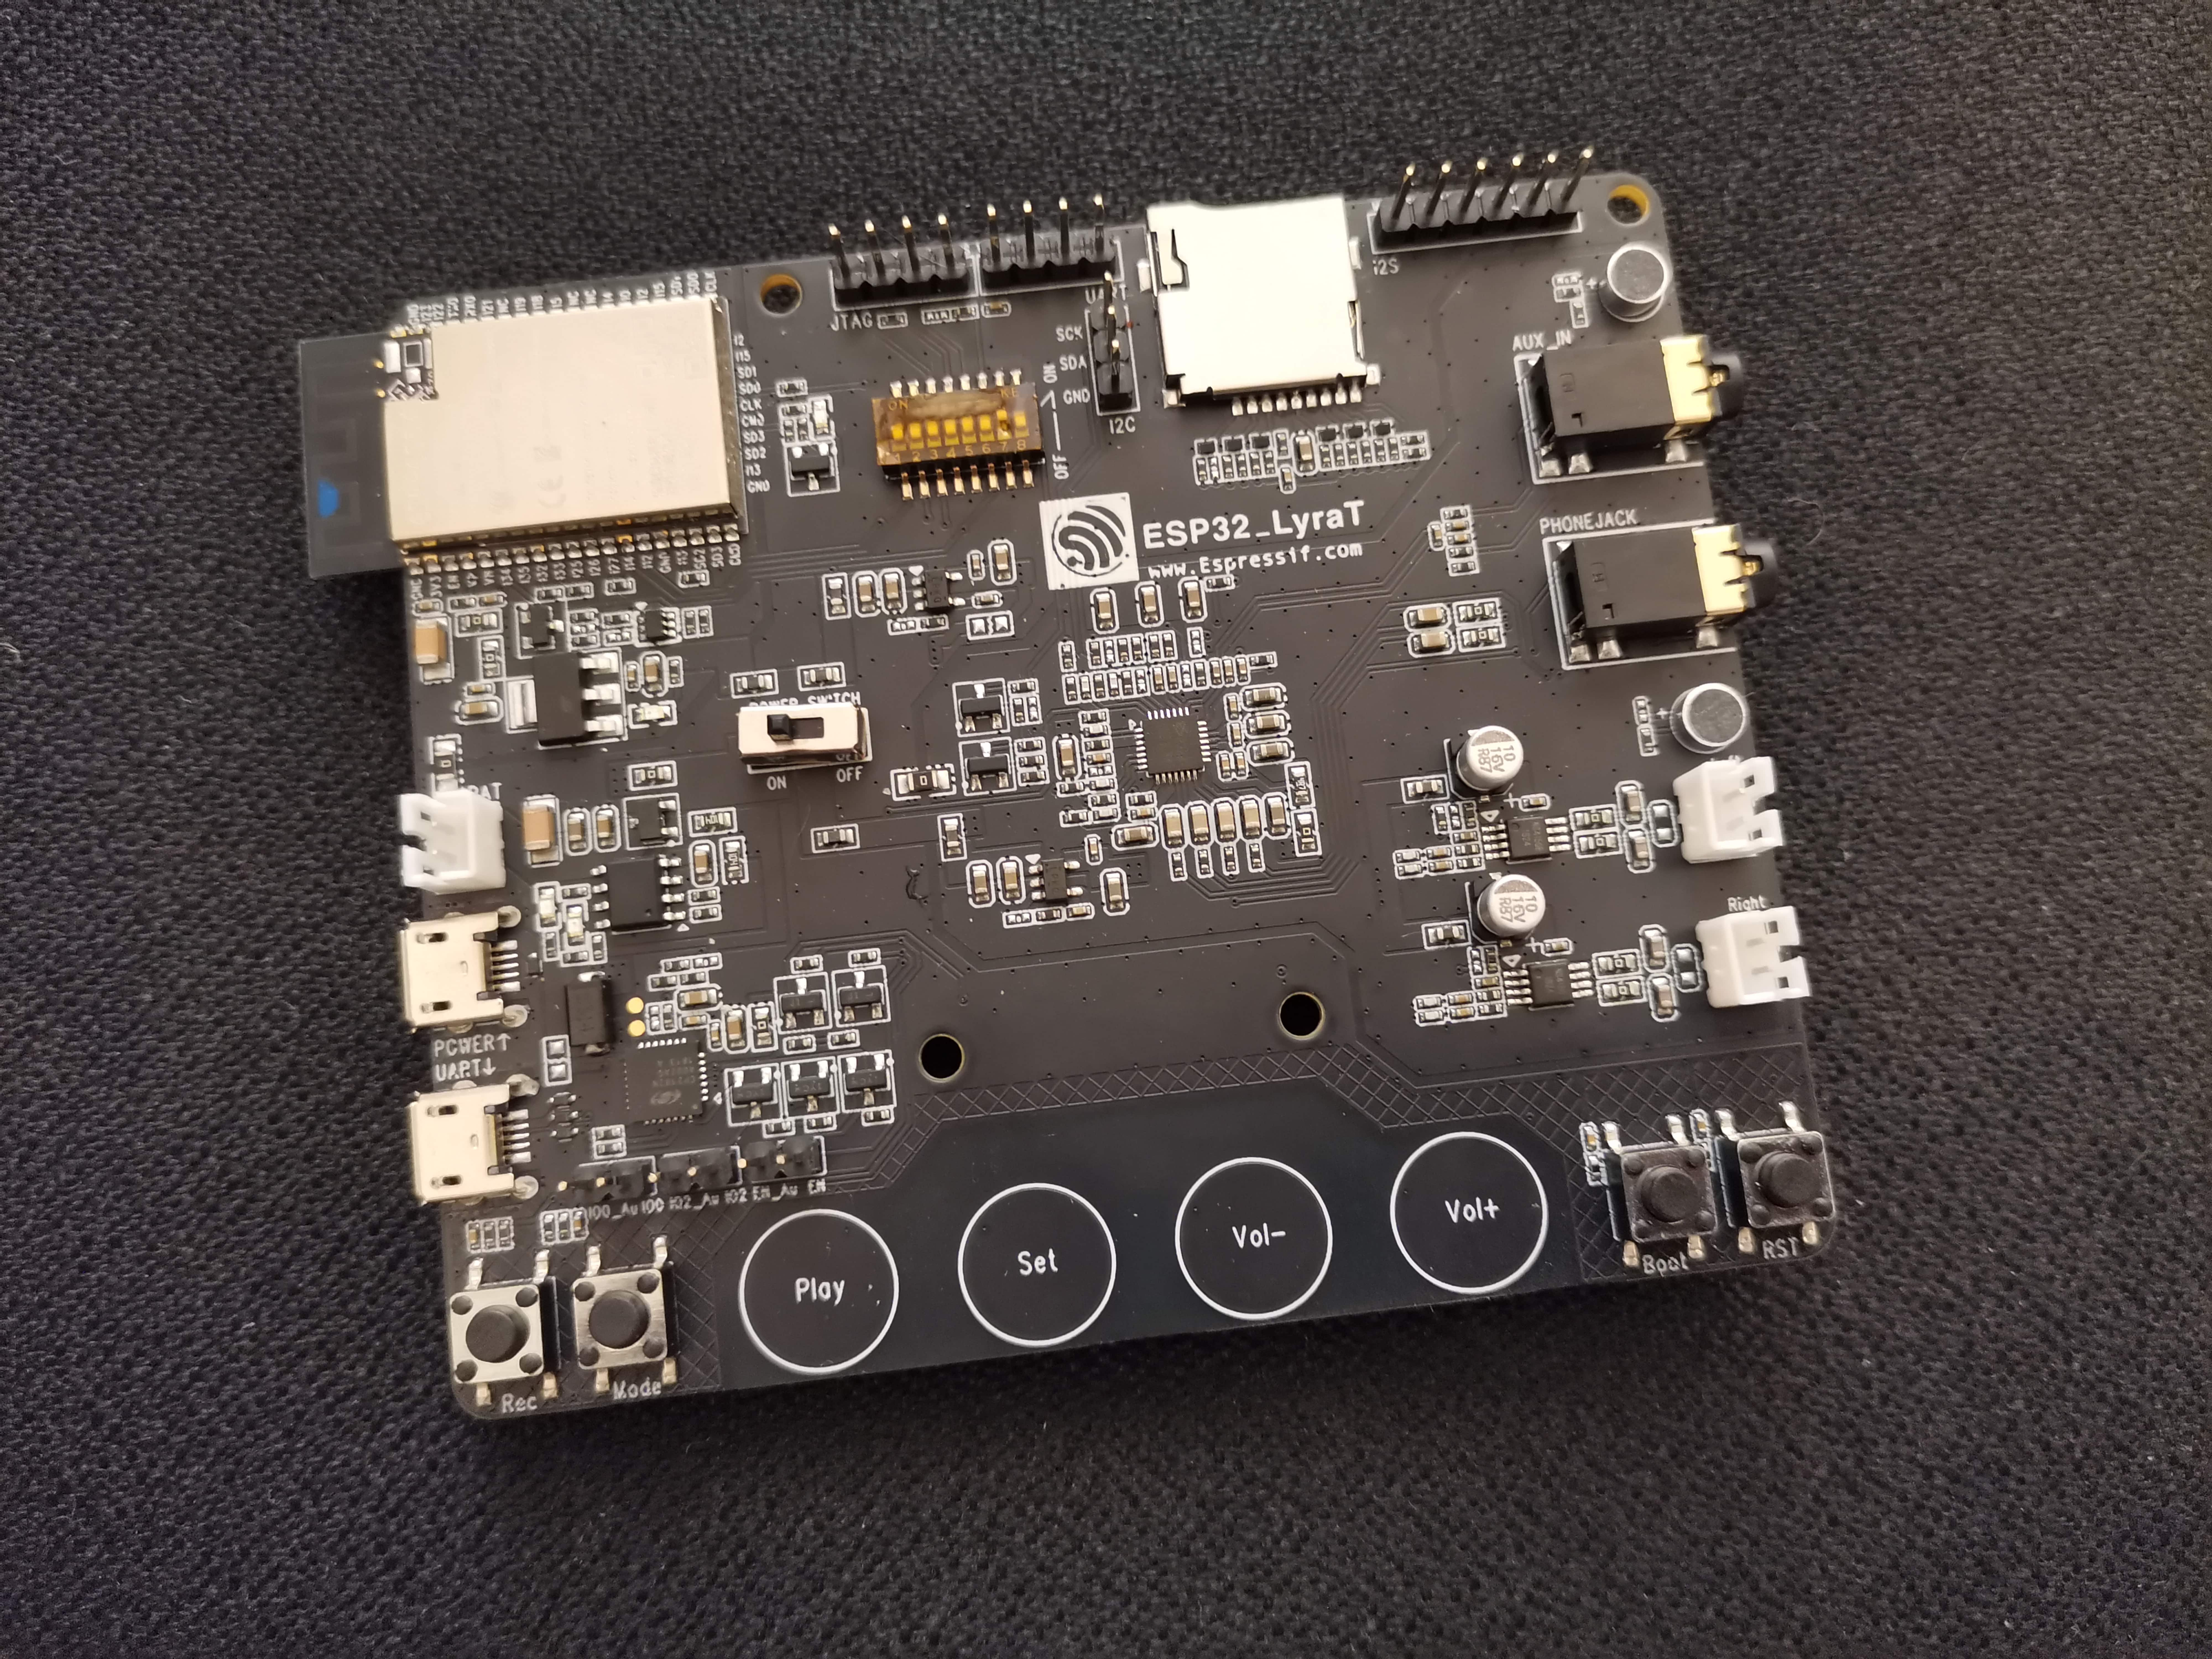
\includegraphics[width=1\linewidth]{images/ESP32-LyraT-1.jpg}
\end{minipage}%
\begin{minipage}{.5\textwidth}
  \centering
  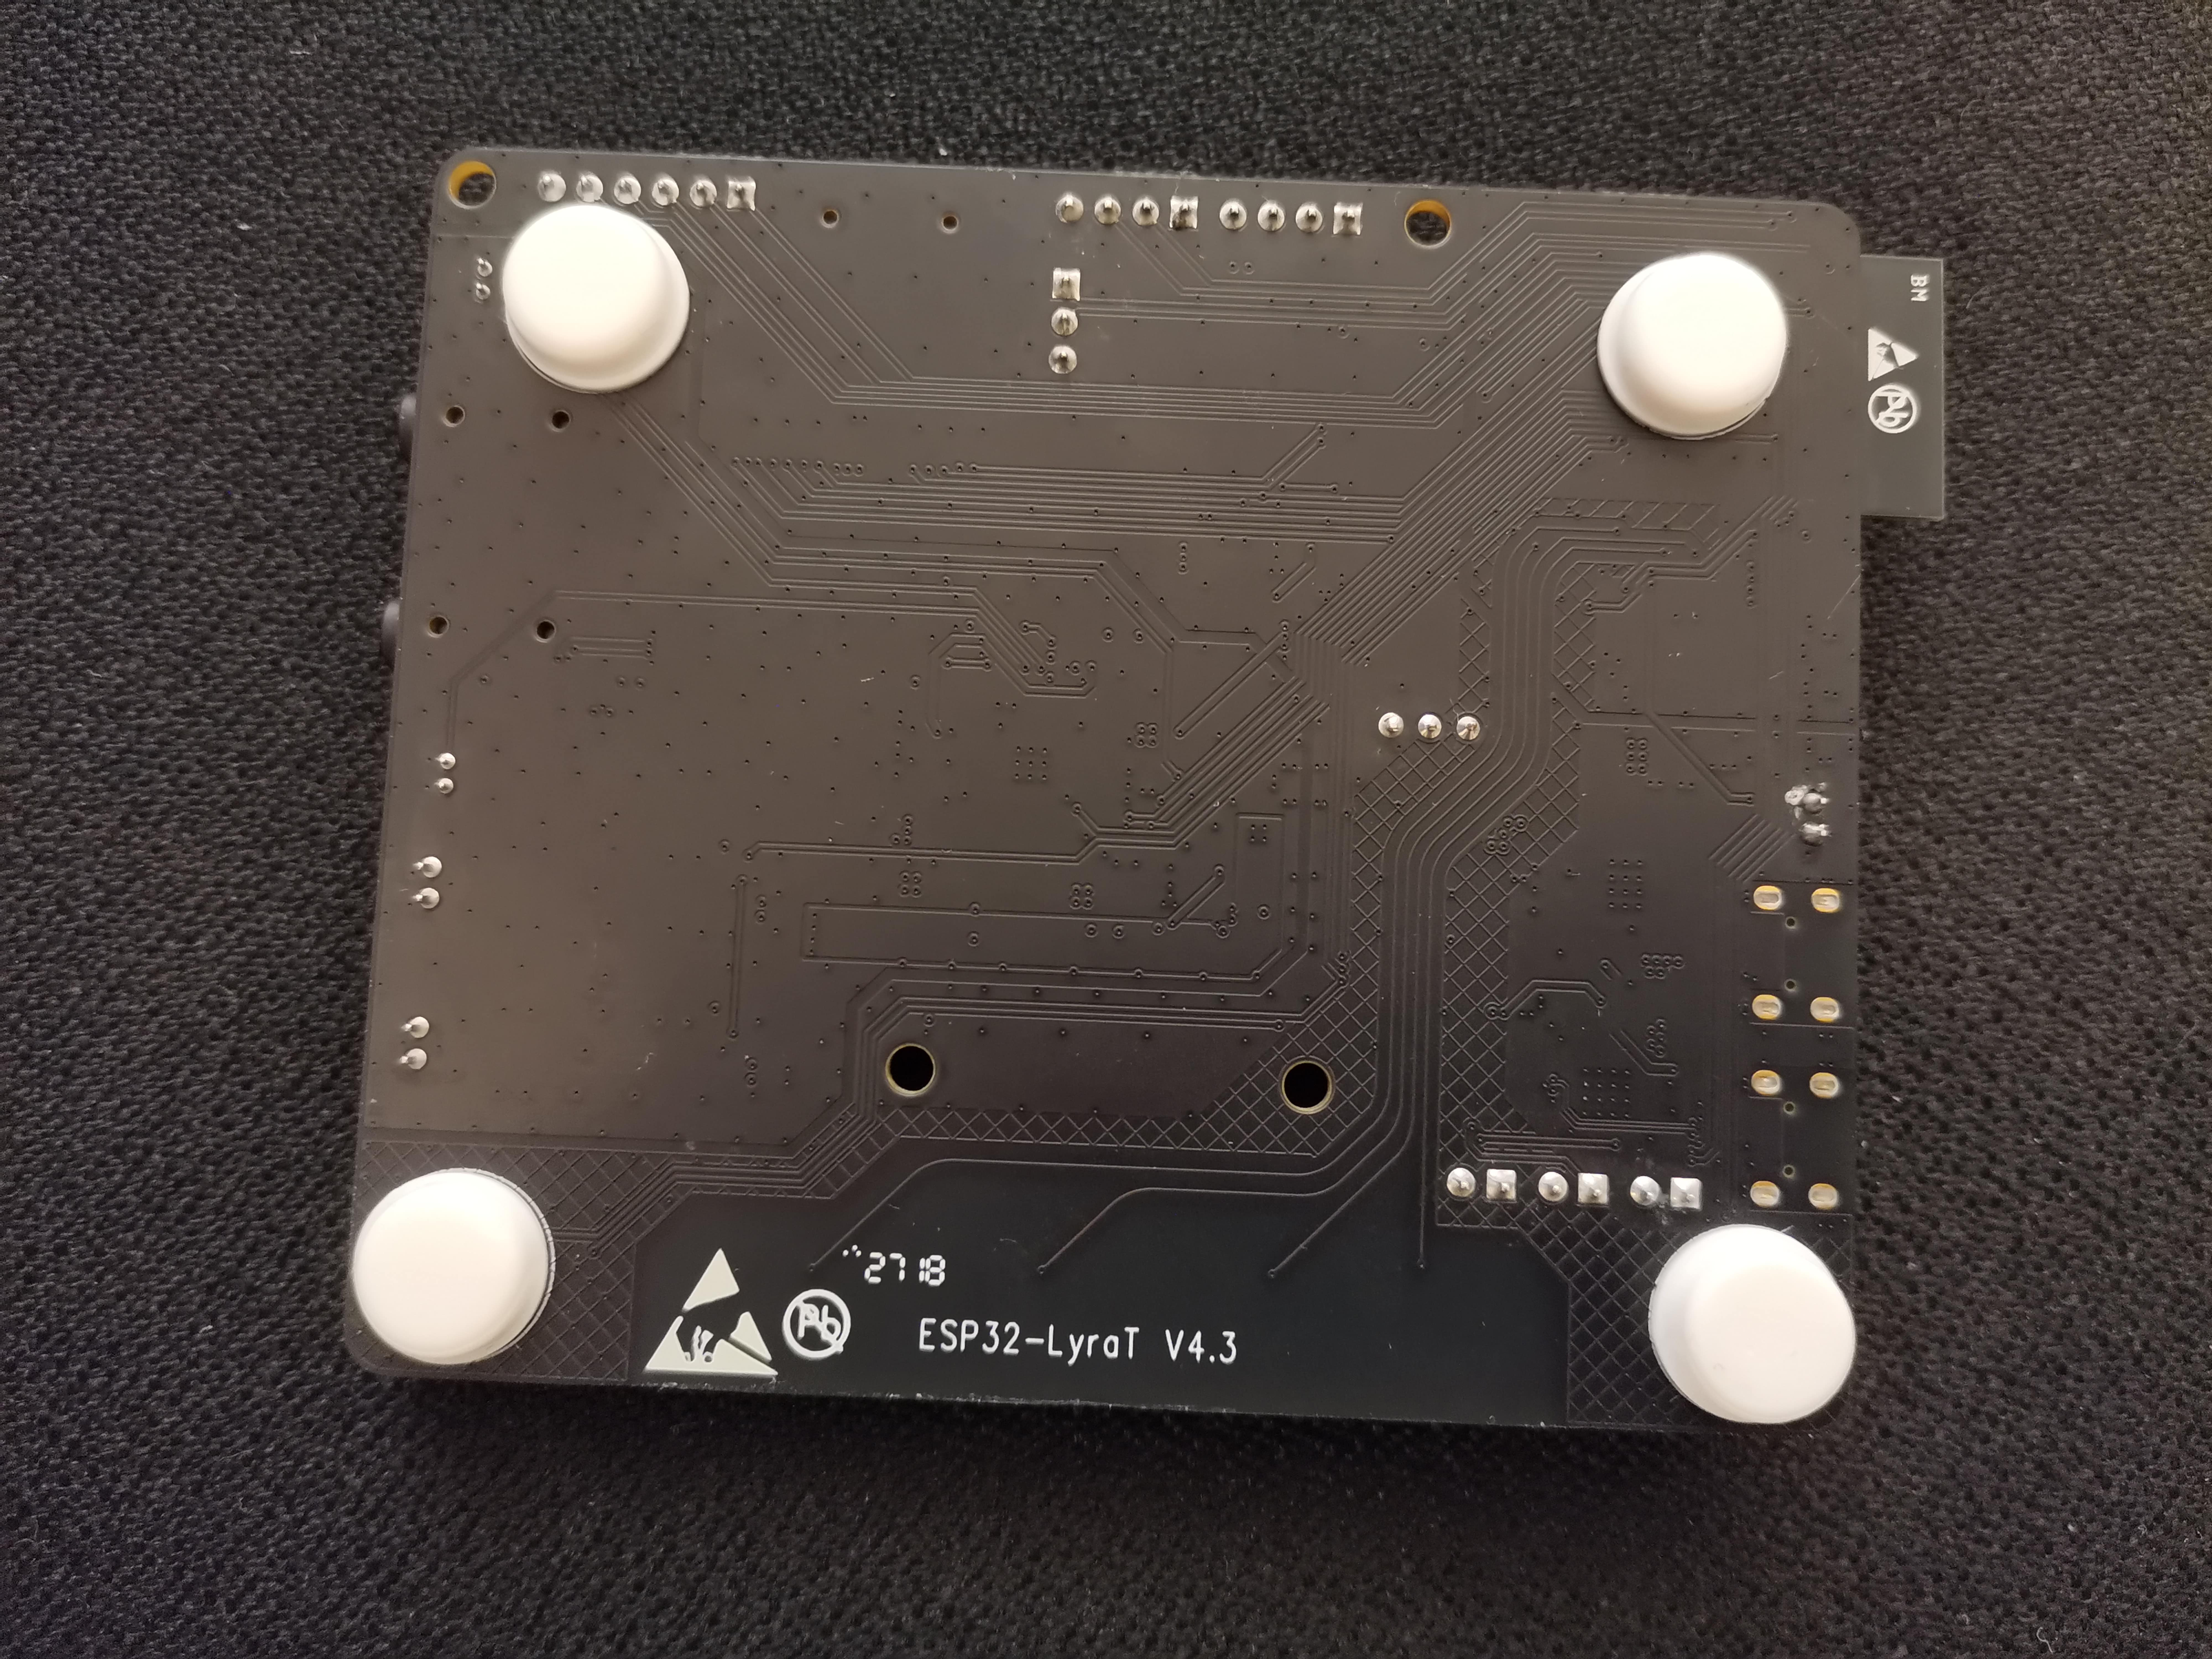
\includegraphics[width=1\linewidth]{images/ESP32-LyraT-2.jpg}
\end{minipage}
\caption{ESP32-LyraT}
\label{esp32-lyrat}
\end{figure}
\fi

It is an audio development board built around ESP32 with additional hardware:
\begin{itemize}
\item	ESP32-WROVER Module
\item	Audio Codec Chip
\item	Dual Microphones on board
\item	Headphone input
\item	2x 3-watt Speaker output
\item	Dual Microphones on board
\item	Dual Auxiliary Input
\item	MicroSD Card slot
\item	Buttons
\item	JTAG
\item	Integrated USB-UART Bridge Chip
\item	Li-ion Battery-Charge Management
\end{itemize}

The main reason for selecting this platform is inbuild external memory of the capacity 8MB. With this size of memory, it should be without any problems to implement selected algorithms. But in reality, only 4MB are able to be used in the implementation, more information can be found in section \ref{esp-memory}. Added with excellent documentation at "docs.espressif.com" it was relatively easy to choose this platform for development.

\bigskip
\noindent
The implementations are the same as reference implementations with my adjustments. What I did is that I tried to port them on ESP32 platform.

%%%%%%%%%%%%%%%%%%%
\subsection{Setup of environment}
First step of development on ESP32 is to set up of environment. This setting I did on Ubuntu 19.4 operating system, starting with downloading of tools:
\begin{lstlisting}[frame=single]
sudo apt-get install git wget libncurses-dev flex bison gperf \
python python-pip python-setuptools python-serial python-click \
python-cryptography python-future python-pyparsing  \
python-pyelftools cmake ninja-build ccache libffi-dev libssl-dev
\end{lstlisting}

\bigskip
\noindent
Add current logged user to group \textit{dialout} because the user needs to get read and write access to the serial port over USB and restart the PC.
\begin{lstlisting}[frame=single]
sudo usermod -a -G dialout $USER
\end{lstlisting}

\bigskip
\noindent
Download software libraries provided by Espressif, Espressif IoT Development Framework (esp-idf), to folder "\$HOME/esp". I used release version 4.1:
\begin{lstlisting}[frame=single]
cd $HOME/esp
git clone -b release/v4.1 --recursive \
https://github.com/espressif/esp-idf.git
\end{lstlisting}
Be \textbf{aware} that all of the setting is related to absolute path "\$HOME/esp". Or copy the whole folder "src/esp" to "\$HOME/esp".

\bigskip
\noindent
Install tools used by "esp-idf" to directory "\$HOME/.espressif":
\begin{lstlisting}[frame=single]
cd $HOME/esp/esp-idf
./install.sh
\end{lstlisting}

\bigskip
\noindent
Last step is to set up environment variables in the terminal where is going to be used "esp-idf":
\begin{lstlisting}[frame=single]
. $HOME/esp/esp-idf/export.sh
\end{lstlisting}
But I added it to file \textit{.bashrc}:
\begin{lstlisting}[frame=single]
echo ". $HOME/esp/esp-idf/export.sh \
	&> /dev/null" >> $HOME/.bashrc
\end{lstlisting}
This way it will be added to every new shell session.

\subsubsection{Build \& Load}
To load application to ESP32-LyraT, one must first build the project. For example, copy the project "src/esp/luov" (in the Diploma thesis sources) to "\$HOME/esp/luov". In this folder it is possible to build it:
\begin{lstlisting}[frame=single]
idf.py -n build
\end{lstlisting}
The switch "-n" will stop treat the warnings as errors.

\bigskip
\noindent
After successful build it is possible to load/flash application to ESP32-LyraT:
\begin{lstlisting}[frame=single]
idf.py -p /dev/ttyUSB0 flash
\end{lstlisting}
The value of the port can be different it depends on to which is ESP32-LyraT connected to.

\bigskip
\noindent
When the loading/flashing starts, it will be waiting for connection from ESP32-LyraT. At that moment hold boot button and press restart button.

\bigskip
\noindent
To check if application is indeed running after loading/flashing, use monitoring system:
\begin{lstlisting}[frame=single]
idf.py -p /dev/ttyUSB0 monitor
\end{lstlisting}
For ESP32-LyraT, when monitoring starts, press restart button.

\bigskip
\noindent
It is possible to combine previous commands together:
\begin{lstlisting}[frame=single]
idf.py -p /dev/ttyUSB0 build flash monitor
\end{lstlisting}

%%%%%%%%%%%%%%%%%%%
\subsubsection{Memory} \label{esp-memory}
Microcontroller ESP32-LyraT has 8MB of external memory (SRAM/SPIRAM). But it is 32-bit processor that means, if external RAM is enabled, only 4MB can be allocated using standard \textit{malloc} calls. To use the region above the 4MB limit, it is possible to use the \textit{himem API}.

\bigskip
\noindent
\textbf{Configuration} - For enabling the external RAM, navigate to "menuconfig $\rightarrow$ Component config $\rightarrow$ ESP32-specific $\rightarrow$ Support for external, SPI-connected RAM $\rightarrow$ SPI RAM config". To access "menuconfig":
\begin{lstlisting}[frame=single]
idf.py menuconfig
\end{lstlisting}

\bigskip
\noindent
\textbf{Stack} - It is possible to change size of the stack for the application. Setting can be found at "menuconfig $\rightarrow$ Component config $\rightarrow$ Common ESP-related $\rightarrow$ Main task stack size".

\bigskip
\noindent
\textbf{Himem} - API which enables access to the remaining memory of external RAM. However, this is done through a bank switching scheme. Configuration can be found at the same place in menuconfig as external RAM.

%%%%%%%%%%%%%%%%%%%
\subsection{Project description}
Base project of esp-idf is composed of the:
\begin{itemize}
\item	build - A folder where the output of build process is stored.
\item	components - A folder which contains subprojects or external projects of the application.
\item	main - A folder which contains source codes of the application. It is also called the \textit{main} component. 
\item	CMakeList.txt - A global setting of the project and starting file for \textit{cmake}. 
\item	sdkconfig - A setting of \textit{menuconfig}.
\item	sdkconfig.default - A default setting of \textit{menuconfig}.
\end{itemize}
But for good convenience I added to this structure a file:
\begin{itemize}
\item	README.md - A file with basic information about build.
\end{itemize}

\noindent
The project can be build by using \textit{make} or \textit{cmake}. For simplicity and recommendation in documentation, also almost every example is written in it, I decided to use \textit{cmake}.

\bigskip
\noindent
Main entry point of application running on ESP32 is function \textit{app\_main}. In provided implementations it can be found in file \textit{main/test.c}.

%%%%%%%%%%%%%%%%%%%
\subsection{LUOV} \label{esp-luov-make}
To make a port of LUOV reference implementation to ESP32, first I needed to create \textit{CMakeList.txt} in folder \textit{main}. This file contains build options for the \textit{main} component.
\begin{lstlisting}[frame=single]
idf_component_register(SRCS INCLUDE_DIRS PRIV_REQUIRES)
\end{lstlisting}
Function is for registering project component to internal build structure of \textit{idf} API.
\begin{itemize}
\item	SRCS  - Files of source codes.
\item	INCLUDE\_DIRS - Paths to header files.
\item	PRIV\_REQUIRES - Components which have to be build before \textit{main} component and then linked to it.
\end{itemize}

\noindent
It is necessary to set up path to \textit{idf} compilator header files otherwise the default, in my case GCC, headers will be used which are incompatible with ESP32.
Last part of this file is block which take care of parsing build flags of project in variable \textit{B\_FLAGS}. 

\bigskip
\noindent
The implementation requires component \textit{XKCP} for PRNG. But how it can be seen in the file \textit{components/XKCP/CMakeList.txt} it only requests few files from the \textit{XKCP} project. That means it is not necessary to build the whole project but only the required parts. This way it will reduce the size of the final application. 

\bigskip
\noindent
One of the important required changes is a change of default value for size of stack to 20000B. This size is sufficient to support all of the stack memory allocation. Also, it needs to enable the use of external memory. Both of the settings are set in \textit{sdkconfig.default}.

\bigskip
\noindent
The reference implementation has implementation (file \textit{rng.c}) of random number generator (RNG) from NIST standard. But this RNG require library \textit{OpenSSL} which by default is not part of the \textit{esp-idf}. I found there is a component \textit{esp-wolfssl} which is embedded SSL library and offers a simple API with OpenSSL compatibility layer. Unfortunately calling initialization function of the \textit{OpenSSL} the ESP32-LyraT will do a segmentation fail. It means that it is not possible to use it.

\bigskip
\noindent
What is possible to do and what I also did, is to change the RNG to hardware RNG of ESP32. But there is condition in which Wi-Fi or Bluetooth needs to be enabled otherwise it can not be considered a true random number generator but only pseudo-random number generator.

\bigskip
\noindent
Implementation can be found in folder \textit{src/esp/luov}. 

\subsubsection{Optimization}
Because this ported implementation of LOUV is fast and has low memory consumption (see chapter \ref{test-and-disk}), I did not try to make any optimization attempts. 

\subsubsection{Memory} \label{esp-luov-memory}
To be able measure the allocated memory in ESP32, I implemented memory measurement with the help of \textit{esp-idf} API. Implementation can be found in file \textit{memory\_measurement.c}.

\bigskip
\noindent
This measurement will create new independent task which periodically ask the ESP32 about internal and external memory status. Because the ESP32 is dual-core processor, the slowdown by this task should be minimal and this should have minimal influence on signing algorithm. But to by sure there is no slowdown, the speed measurement was taken without this memory measurement.

\bigskip
\noindent
To enable this functionality, the following flag needs to be set:
\begin{itemize}
\item	MEM\_MEASUREMENT
\end{itemize}

%%%%%%%%%%%%%%%%%%%
\subsection{Rainbow}
To make a port of Rainbow reference implementation to ESP32, I proceeded in the same way as for the LUOV ESP32 implementation. That means I created \textit{CMakeList.txt} in folder \textit{main} with the same formalities as \textit{CMakeList.txt} for LUOV, see section \ref{esp-luov-make}. The most eye catching difference is set up of different kinds of \textit{malloc}, see section \ref{esp-rb-memory} for more information.

\bigskip
\noindent
The implementation requires component \textit{wolfssl} for PRNG. In this case is build the whole \textit{esp-wolfssl} project which is simply added through \textit{PRIV\_REQUIRES} in \textit{main/CMakeList.txt}. Here is important to mention that Rainbow reference implementation contains two PRNG (see \textit{utils\_prng.c}). One from NIST standard, it is the same RNG as in LUOV reference implementation, and second PRNG which use hash SHA function. Because the RNG form NIST standard was not possible for me to run on ESP32-LyraT, I change it to second PRNG and  I deleted from source codes the implementation of the first.

\bigskip
\noindent
The source codes also require RNG which I changed to hardware RNG of ESP32, it is the same change as in LUOV ESP32 implementation (see \textit{rng.c}).

\bigskip
\noindent
The default value for size of stack I set up to value 5000B. Because this value is sufficient to support all of the Rainbow stack allocation memory. Setting is set up in \textit{sdkconfig.default} with enabled external memory to get access to external 4MB RAM.

\bigskip
\noindent
Implementation can be found in folder \textit{src/esp/rb}. 

\subsubsection{Optimization} \label{rb-opti}
I did two memory optimizations of Rainbow implementation for ESP32:
\begin{itemize}
\item	First I found potential big allocation of memory and switch them from stack to heap. Candidates to change were temporary helpful variables of keys (\textit{sk\_t}) in computation of keys from seeds.

\item	Second I created \textit{my\_ESP\_malloc} and \textit{my\_ESP\_free} functions, see \ref{esp-rb-memory}. With these I found that temporary variables (for example \textit{sk\_t* tempQ}) were using lot of memory but in reality only needed a part of the key structure. See commit \textit{"ESP - RB memory reduction in cyclic generation"}, hash \textit{"1609d70c"} for details of optimization.
\end{itemize}

With these two optimizations there was already enough memory and I was able to run \textit{\_RAINBOW256\_92\_48\_48} implementation in compressed form. I was also able to run the same implementation in cyclic form but there is same kind of bug and it was making segmentation fault. I am suspecting that it is the same bug 
which causes failure of signature verification.

\subsubsection{Memory} \label{esp-rb-memory}
To be able to better measure the allocated memory in ESP32, there is the same memory measurement implementation as in LUOV ESP32 \ref{esp-luov-memory}, which can be enabled by flag:
\begin{itemize}
\item	MEM\_MEASUREMENT
\end{itemize}

Because I needed better technique for memory allocation on heap, I created my own allocation information table. It is simple small array, I expect small number of allocation at one point at a time, which holds information of pointer and its size.
It can be enabled by flag:
\begin{itemize}
\item	MY\_ESP\_MALLOC
\end{itemize}
When this flag is set, it will switch all \textit{aligned\_alloc} to \textit{my\_ESP\_malloc} and \textit{free} to \textit{my\_ESP\_free} and every time when there is allocation od deallocation it will print its information.
This information table helped me to identify potential places in source code of RB for memory optimization. For implementation details see file \textit{malloc.c}.

\bigskip
\noindent
The reference implementation use \textit{aligned\_alloc} function for allocation of memory but ESP32 with toolchain 8.2 which I am using has issue with this function and it is not possible to use for now. That is the reason why I change it to classic \textit{malloc} function.

%%%%%%%%%%%%%%%%%%%%%%%%%%%%%%%%%%%%%%%%%%%%
\newpage
\section{Conventional algorithms}
These selected conventional algorithms were also implemented on microcontroller ESP32-LyraT for the possibility of comparison with LOUV and RB. These two algorithms are one of the most typical and most used in computer for signature schemes, that means there exist very good software implementations with hardware acceleration on ESP32 chip. 

\bigskip
\noindent
Both of the selected algorithms are implemented, using the esp-idf API, in similar way like previous implementations in this thesis on ESP32. That means their entry point is in file \textit{test.c} which has similar structure to others \textit{test.c} files in previous description. The main difference is in private and public keys which are now in the form of \textit{context} relative to algorithm.

\subsection{RSA}
Test implementation of RSA starts with initialization of context:
\begin{lstlisting}[frame=single]
mbedtls_rsa_context ctx;
mbedtls_rsa_init(&ctx,MBEDTLS_RSA_PKCS_V15,0);
\end{lstlisting}

\noindent
Second step is generation of keypair:
\begin{lstlisting}[frame=single]
mbedtls_rsa_gen_key(&ctx,coap_prng_impl,NULL,KEY_SIZE,EXPONENT);
\end{lstlisting}

\noindent
Generation \textit{hash} of message $m$:
\begin{lstlisting}[frame=single]
mbedtls_sha256(m,message_size,hash,0);
\end{lstlisting}

\noindent
Sign \textit{hash} and put signature to \textit{sm}:
\begin{lstlisting}[frame=single]
mbedtls_rsa_pkcs1_sign(&ctx,coap_prng_impl,NULL,
			MBEDTLS_RSA_PRIVATE,MBEDTLS_MD_SHA256,
			0,hash,sm);
\end{lstlisting}

\noindent
Verify signature \textit{sm} of \textit{hash}:
\begin{lstlisting}[frame=single]
mbedtls_rsa_pkcs1_verify(&ctx,coap_prng_impl,NULL,
			MBEDTLS_RSA_PUBLIC,MBEDTLS_MD_SHA256,
			0,hash,sm);
\end{lstlisting}

\bigskip
\noindent
The implementation can be set with flags:
\begin{itemize}
\item	KEY\_SIZE - Size of public key in bits.
\item 	EXPONENT - Public exponent to use.
\item 	MEM\_MEASUREMENT  - Enable memory measurement.
\end{itemize}

%%%%%%%%%%%%%%%%%%%
\subsection{ECDSA}
Test implementation of ECDSA is very similar to RSA. It starts with initialization of context:
\begin{lstlisting}[frame=single]
mbedtls_ecdsa_context ctx;
mbedtls_ecdsa_init(&ctx);
\end{lstlisting}

\noindent
Second step is generation of keypair:
\begin{lstlisting}[frame=single]
mbedtls_ecdsa_genkey(&ctx,EC_CURVE,coap_prng_impl,NULL);
\end{lstlisting}

\noindent
Generation \textit{hash} of message $m$:
\begin{lstlisting}[frame=single]
mbedtls_sha256(m,message_size,hash,0);
\end{lstlisting}

\noindent
Sign \textit{hash} and put signature to \textit{sm}:
\begin{lstlisting}[frame=single]
mbedtls_ecdsa_write_signature(&ctx,MBEDTLS_MD_SHA256,hash,
			hash_len,sm,&smlen,coap_prng_impl,NULL);
\end{lstlisting}

\noindent
Verify signature \textit{sm} of \textit{hash}:
\begin{lstlisting}[frame=single]
mbedtls_ecdsa_read_signature(&ctx,hash,hash_len,sm,smlen);
\end{lstlisting}

\bigskip
\noindent
The implementation can be set with flags:
\begin{itemize}
\item	EC\_CURVE\_BITS  - Number of bits for elliptic curve.
\item 	MEM\_MEASUREMENT  - Enable memory measurement.
\end{itemize}


%%%%%%%%%%%%%%%%%%%%%%%%%%%%%%%%%%%%%%%%%%%%
%%%%%%%%%%%%%%%%%%%%%%%%%%%%%%%%%%%%%%%%%%%%
\chapter{Testing and discussion} \label{test-and-disk}
This chapter contains measurement and testing of algorithms, their comparison and discussion about their implementation. It mainly focuses on time and memory complexity of the selected algorithms and possible usability in an embedded environment.

\section{PC}
The reference implementations with my adjustments were tested on computer with parameters:
\begin{itemize}
\item OS: Ubuntu 19.4
\item CPU: Intel Core i5-7300HQ
\item Clock Speed: 2.50GHz
\item RAM: 8 GB
\item Number of cores: 4
\item Compilator: GCC 8.3.0
\end{itemize}

\bigskip
\noindent
Every measurement was done on message of size 10000B and 10 times. The final result in the graphs below is average value.

\bigskip
\noindent
Main goal of this measurements and implementations is to have comparable data of reference implementations of LUOV and RB on PC because in reference materials there are measured on different processors and only in number of processor cycles. I chose to make the measurement of time (in seconds) and memory consumption (in bytes).

\bigskip
\noindent
The solutions are compiled with the same (default) setting with flag \textit{-std=c99}.

\subsection{Signature variants}
For measurement I selected the reference signature variants. The first number indicate finite field $\mathbb{F}_{n}$, second is number of vinegar variables, third is number of oil variables and the fourth (at RB) is number of oil variables in second layer. Dividing by security categories there are:

\bigskip
\noindent
Category II:
\begin{itemize}
\item Luov-47-42-182
\item Luov-7-57-197
\item Rb-16-32-32-32 - and its variants
\end{itemize}

\noindent
Category IV:
\begin{itemize}
\item Luov-61-60-261
\item Luov-7-83-283
\item Rb-256-68-36-36 - and its variants
\end{itemize}

\noindent
Category V:
\begin{itemize}
\item Luov-79-76-341
\item Luov-7-110-374
\item Rb-256-92-48-48 - and its variants
\end{itemize}

\noindent
Each of the categories represent a difficulty through how many hardware gates needs to be used to be able to break the security variant.\cite{L-NIST-STANDARD} Overview:
\begin{table}[H]
\centering
\begin{tabular}{|c|c|c|c|}
\hline
Category & Log\textsubscript{2} classical gates & Log\textsubscript{2} quantum gates  & Ex. of alg.\\ \hline
I         & 143                    & 130/106/74    & AES-128     \\ \hline
II        & 146                    &                      & SHA3-256  \\ \hline
III       & 207                    & 193/169/137  & AES-192     \\ \hline
IV        & 210                    &                     & SHA3-384   \\ \hline
V         & 272                    & 258/234/202 & AES-256      \\ \hline
VI        & 274                    &                     & SHA3-512   \\ \hline
\end{tabular}
\caption{NIST security categories}
\end{table}

\noindent
For the quantum gates, there is also parameter \textit{MAXDEPTH} of $2^{40}$, $2^{64}$, $2^{96}$ which represent fixed running time, or circuit depth. The reason for this parameter is Grover’s algorithm.

\bigskip
\noindent
An algorithm meets the requirements of a specific security category if the best known attack uses more resources (gates) than are needed to solve the reference problem.

\bigskip
\noindent
With regard to the LUOV parameters, finite field of size 7 is selected because of small size of generated signature but the size of public key is quite big. The schemes which do not have finite field of size 7 are selected because of small public key.

%%%%%%%%%%%%%%%%%%%
\subsection{Time complexity} \label{time-complex-pc}
The next two graphs display individual stages of the signature scheme and time it takes to complete each of the stages. Namely generation, signing and verification. For time measurement I used \textit{clock\_t} from standard header \textit{time.h}. 
\begin{figure}[H]
\centering
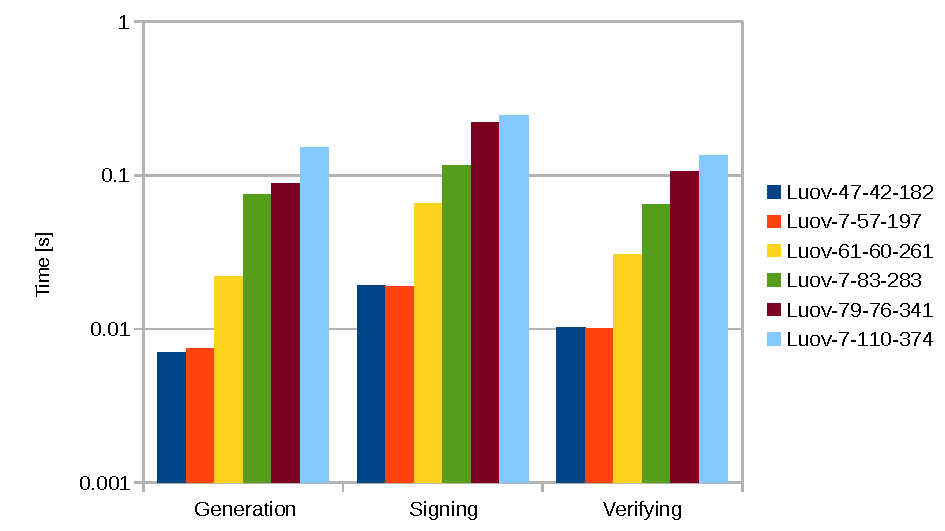
\includegraphics[width=13cm,height=7cm]{images/pc-luov.pdf}
\caption{Comparison of LUOV on PC}
\label{pc-luov}
\end{figure}

\noindent
How it can be seen on \ref{pc-luov} the stronger the security the more of time is needed for the computation which is the expected result. About the generation stage, the shorter the public key the fastest it is, the same is true for the signing and verifying stages which are again expected results.

\bigskip
\noindent
On a graph \ref{pc-rb}, it is possible to see that generating the public key (\textit{cyc} versions) and private key (\textit{com} versions) from the seed is really slow operation. It can be especially seen on signing of \textit{com} variants where the signing stage can be up to 85 times slower (maybe even more) than the classic variants. For the verifying stage is also the fastest then classic variant because there is no generation from the seed.

\begin{figure}[H]
\centering
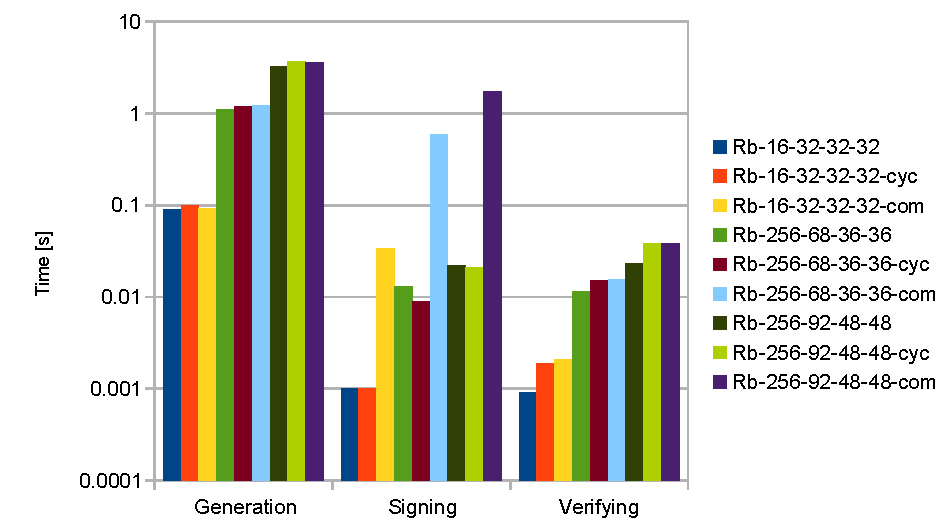
\includegraphics[width=13cm,height=7cm]{images/pc-rb.pdf}
\caption{Comparison of RB on PC}
\label{pc-rb}
\end{figure}

\noindent
Next graph \ref{pc-all} is comparison of LUOV and RB implementation. I only compare the \textit{com} versions of RB with LUOV with short public keys. I selected this LOUV variant because it is faster and this RB variant because it also (like LUOV) generate public and private keys from the seed.
There is not the generation stage because on \ref{pc-luov} and \ref{pc-rb} is very well visible that generation times of RB are much slower than LOUV. 

\begin{figure}[H]
\centering
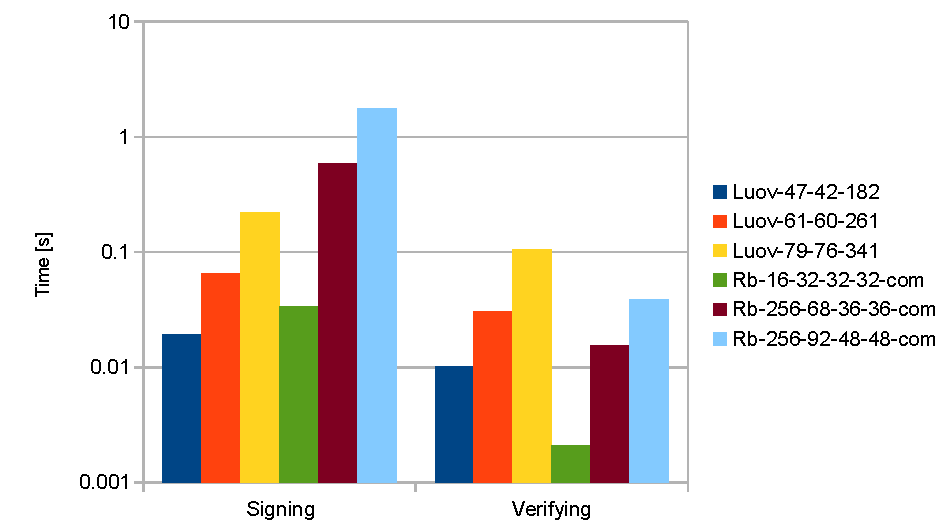
\includegraphics[width=13cm,height=7cm]{images/pc-all.pdf}
\caption{Comparison of PC implementations}
\label{pc-all}
\end{figure}

\noindent
How it can be seen \ref{pc-all} the LOUV implementation is faster at signing but slower at verifying.

%%%%%%%%%%%%%%%%%%%
\subsection{Memory complexity}
Memory complexity deals with the allocation of RAM on heap for the signature schemes. The required memory on stack I did not measure because compare to heap it is negligible (in the magnitude of a few kilobytes). I measured PC implementations with the help of Valgrind. Specifically, with the help of tool \textit{Massif} which is a heap profiler:
\begin{lstlisting}[frame=single]
valgrind --tool=massif ./test
\end{lstlisting}

\noindent
To get a human readable output it needs to be used with:
\begin{lstlisting}[frame=single]
ms_print massif.out.*
\end{lstlisting}
\noindent
From its output I created next few graphs which show the maximum memory allocation (in bytes) over the whole run of test application. 

\bigskip
\noindent
On graph \ref{mem-pc-luov} is visible memory allocation of LUOV. It shows an expected result which is with higher security category the more memory is needed. Also is visible that LOUV variants with shorter public key needs less resources.

\begin{figure}[H]
\centering
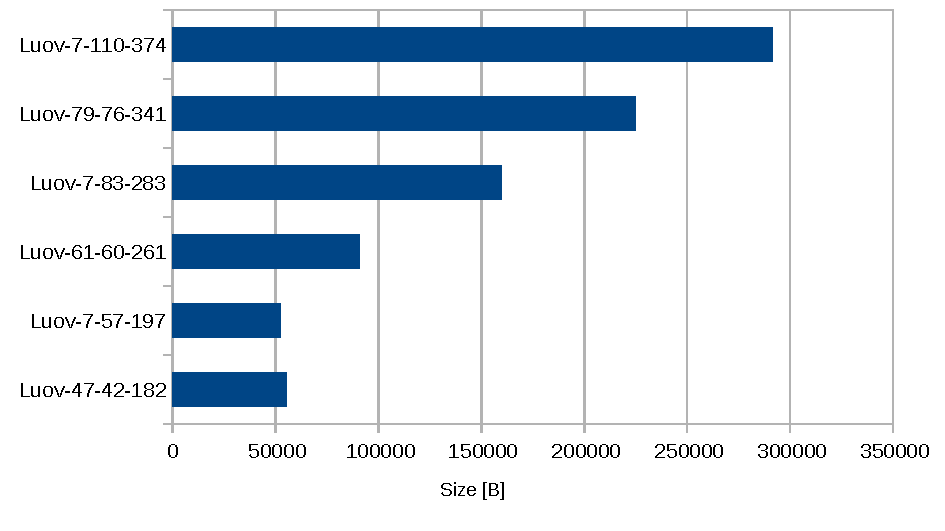
\includegraphics[width=13cm,height=7cm]{images/mem-pc-luov.pdf}
\caption{Memory requirement of LUOV on PC}
\label{mem-pc-luov}
\end{figure}

\noindent
Next is graph \ref{mem-pc-rb} of RB memory allocation. On it is shown again that the higher security category the more resource it needs, which is expected result. But to my surprise the \textit{com} variants of Rainbow need less RAM allocation compared to classic and \textit{cyc} variants. The only explanation I can think of is, which can explain this behavior, is the generation of private key from the seed. That is the main difference compared to other variants.
\begin{figure}[H]
\centering
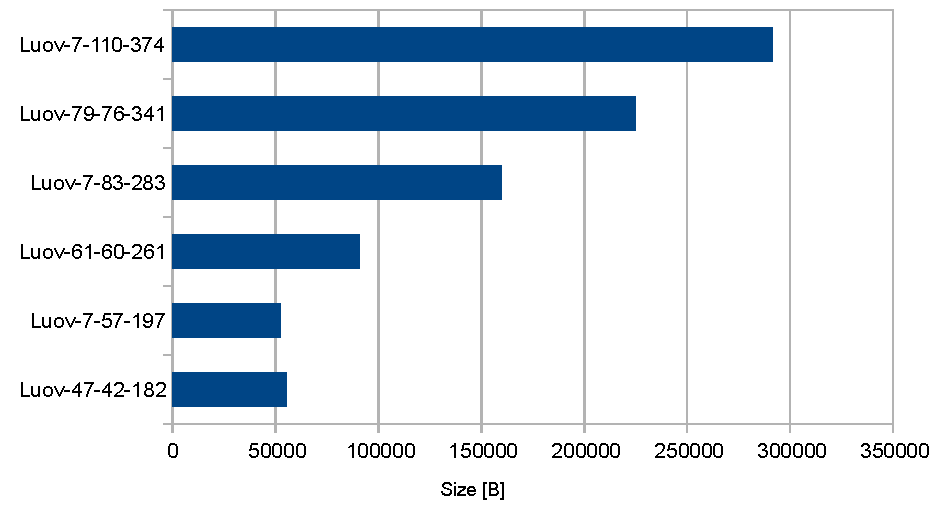
\includegraphics[width=13cm,height=7cm]{images/mem-pc-rb.pdf}
\caption{Memory requirement of RB on PC}
\label{mem-pc-rb}
\end{figure}

\begin{figure}[H]
\centering
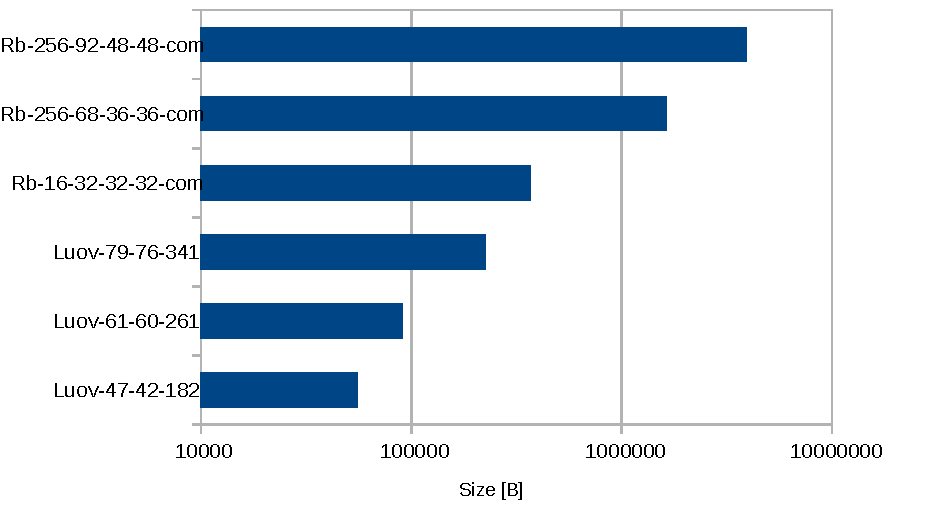
\includegraphics[width=13cm,height=7cm]{images/mem-pc-all.pdf}
\caption{Comparison of PC implementations}
\label{mem-pc-all}
\end{figure}

\noindent
Last graph of memory complexity section is graph \ref{mem-pc-all} of comparison between LUOV and Rainbow. There is shown that LUOV takes a lot less memory resources than RB.  This behavior I contribute to implementation specifics (code programming, optimization and memory handling) which are much more better then in Rainbow implementation.

%%%%%%%%%%%%%%%%%%%
\subsection{Conclusion note}
The measured values show that the reference implementation of LOUV is almost better in everything. It is faster, has smaller memory imprint and has simpler implementation.

\bigskip
\noindent
The only thing in which is Rainbow better is verification of signature (how can be seen on graph \ref{pc-all}) but that is implication from signature size which is shorter than LUOV, for more details see section \ref{key_sign}.

\bigskip
\noindent
From the point of usability, the Rainbow implementation is only optimal if lot of signature verification needs to be done or if there is lot of very short messages then shorter signature can speed up the computational means, for example the network communication.

\bigskip
\noindent
But I do not recommend this implementation of RB because there seem to by some kind of implementation bug. It can be seen on \textit{cyc} variant of RB where verification of signed message reports that it is an invalid signature.

\bigskip
\noindent
If I was faced with the choice of the selection of one of these implementations for general use. I would select the LUOV implementation because, how was already mentioned, it is faster, smaller and do not contains any bug (at least I did not find any).

%%%%%%%%%%%%%%%%%%%%%%%%%%%%%%%%%%%%%%%%%%%%
\newpage
\section{ESP32}
ESP32 implementations were tested and ported on ESP32-LyraT microcontroller, specification of the microcontroller can be found in section \ref{ESP32_impl}. The reason for port is to test the behavior of the selected algorithms in IoT environment or at least as close as possible to it.

\bigskip
\noindent
Every measurement was done on message of size 1000B and 10 times. The final result in the graphs below is average value.

\subsection{Signature variants}
Variants of signature schemes were selected same as in PC section. But there are some changes. Dividing by security categories there are:

\bigskip
\noindent
Category II:
\begin{itemize}
\item Luov-47-42-182
\item Luov-7-57-197
\item Rb-16-32-32-32 - and its variants
\end{itemize}

\noindent
Category IV:
\begin{itemize}
\item Luov-61-60-261
\item Luov-7-83-283
\item Rb-256-68-36-36 - and its variants
\end{itemize}

\noindent
Category V:
\begin{itemize}
\item Luov-79-76-341
\item Luov-7-110-374
\item Rb-256-92-48-48-com
\end{itemize}

\noindent
In category V there is only \textit{com} variant of RB scheme because the other variants (classic and \textit{cyc}) I was not able to make to run because of limited RAM.

\bigskip
\noindent
I did few memory optimizations in RB scheme, it can be found in section \ref{rb-opti}. These optimizations reduce kind of a lot of memory but when I try to run \textit{Rb-256-92-48-48-cyc} variant I get a segmentation fault. This behavior I attributed to a bug in the implementation where the signature is failing. 

%%%%%%%%%%%%%%%%%%%
\subsection{Time complexity}
Like in the PC measurement before, section \ref{time-complex-pc}, next graphs display individual stages of the signature scheme and time it takes to complete each of the stages. For time measurement I also used \textit{clock\_t} from standard header.

\bigskip
\noindent
On graph \ref{time-luov} is comparison of LUOV times which it takes for each of the stages. It can be seen that higher the security category the more time for completion of the stage is needed. That is expected result like on the PC implementations but some of the times is now in the periods around of 10 seconds. Especially \textit{Luov-7-110-374} or generally the whole security category V is with these time periods unusable in the moment when a lot of messages need to be signed or verified.

\bigskip
\noindent
Also, category IV takes a lot of time but the LUOV variant \textit{Luov-61-60-261}, I think is pretty fast enough on ESP32-LyraT and can be used for common signature scheme. As a category IV it can provide very high security for IoT devices but it has one disadvantage and that is a large signature.

\bigskip
\noindent
The variants \textit{Luov-47-42-182} and \textit{Luov-7-57-197} of security category II can be fast on embedded devices and it puts them at the forefront of the other LUOV signature variants.

\bigskip
\begin{figure}[H]
\centering
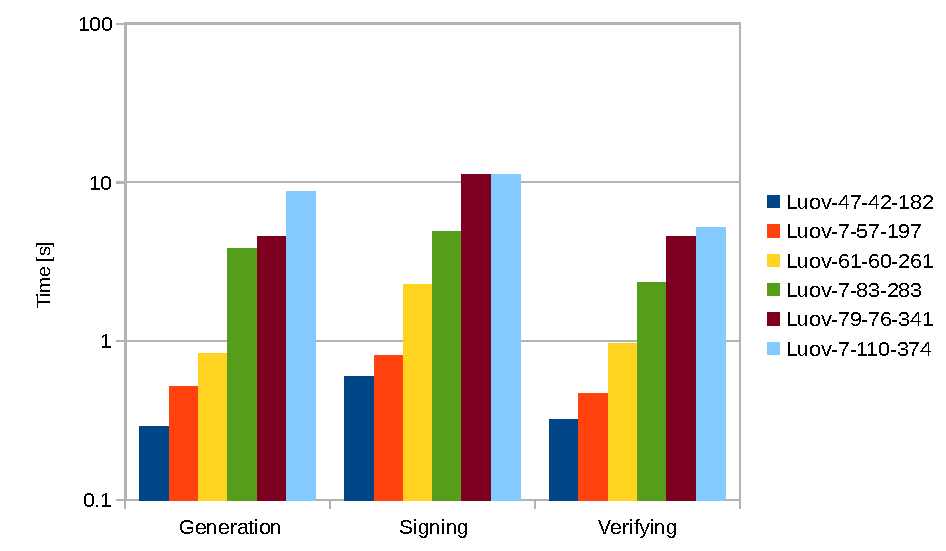
\includegraphics[width=13cm,height=7cm]{images/time-luov.pdf}
\caption{Comparison of LUOV on ESP32}
\label{time-luov}
\end{figure}

Next graph \ref{time-rb} is comparison of times of Rainbow scheme. There it can be seen that generation of the public and private keys is very slow but in practical in the most use cases this step needs to be done only once, therefore it has little influence.

\bigskip
\noindent
It can also be seen that signing and verifying stages do not belong to a fast operations. Especially the \textit{com} versions which are really slow. There is very well visible that generating public and private keys from the seed is not good idea from time point of view. And if there was no generation then there will be very big speedup as can be seen on comparison of \textit{Rb-256-68-36-36} and \textit{Rb-256-68-36-36-com}.

\bigskip
\noindent
Like in LOUV scheme before also in RB scheme is the best variant from security category II, the variant \textit{Rb-16-32-32-32}. Which has more than enough security for the common communication in IoT devices.

\begin{figure}[H]
\centering
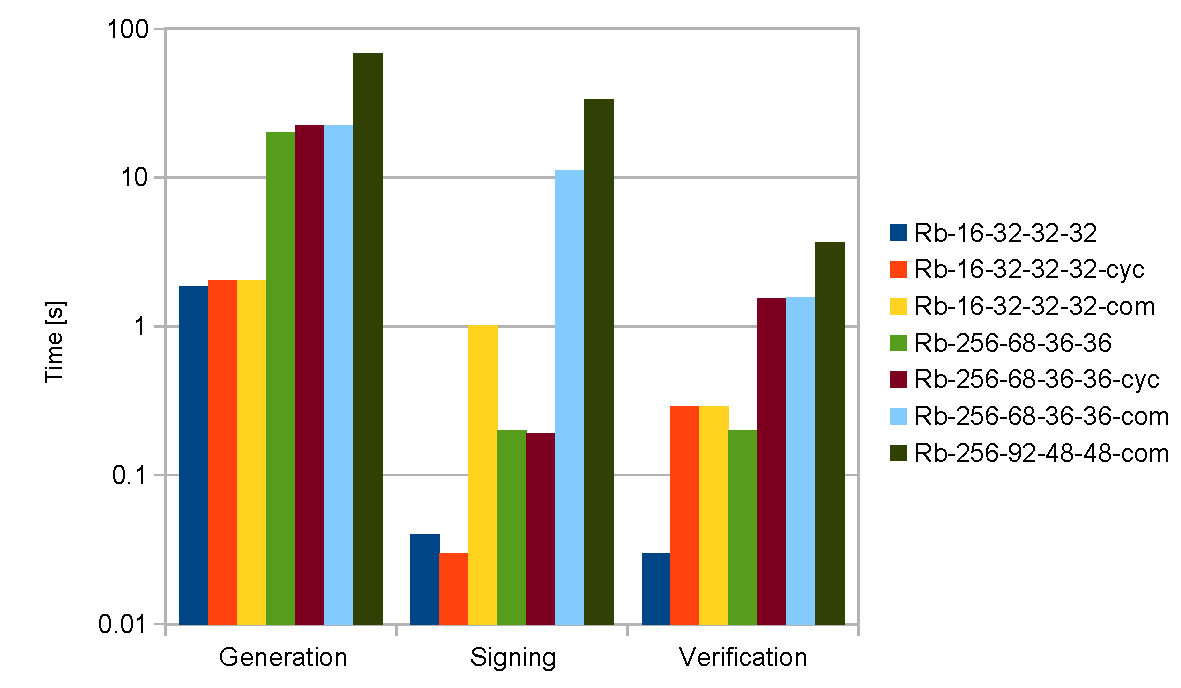
\includegraphics[width=13cm,height=7cm]{images/time-rb.pdf}
\caption{Comparison of RB on ESP32}
\label{time-rb}
\end{figure}

\noindent
Last graph \ref{time-both} of this section is comparison between LUOV and RB. It is only comparison between LOUV variants with shorter public key and RB \textit{com} variants. The reasons for this selection of signature schemes variants are in section \ref{time-complex-pc}.

\bigskip
\noindent
On this graph can be seen that LUOV variants are faster in signing and RB variant are faster in verification process, except the \textit{Rb-256-68-36-36-com} which got slowdown. There is no comparison of generation stage because LOUV is clearly better in every security category.

\bigskip
\noindent
If I compare the ESP32 graphs of time results with PC implementations I can see similar shapes. That means there are no big mistakes in my port of implementation on ESP32. Also is visible that verifying stage of all variants of RB got slowdown compared to PC implementations.

\begin{figure}[H]
\centering
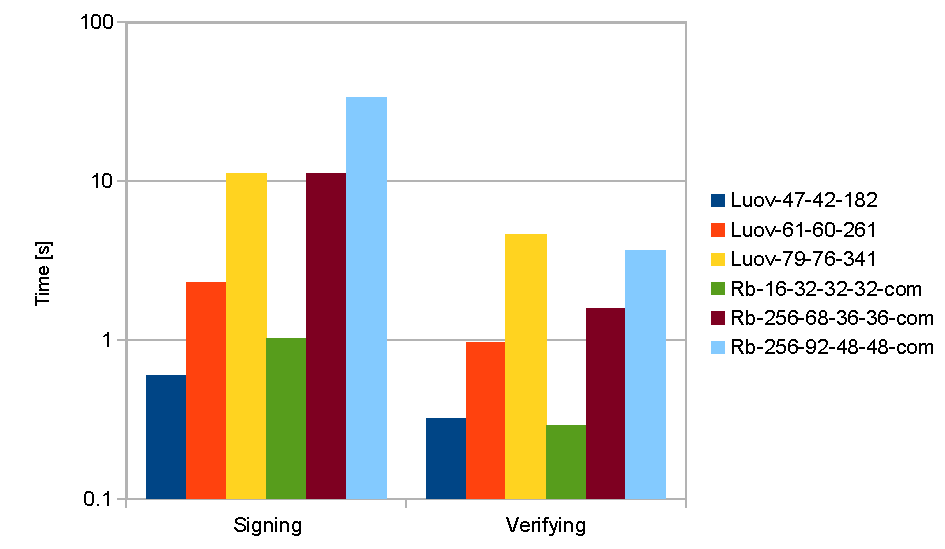
\includegraphics[width=13cm,height=7cm]{images/time-both.pdf}
\caption{Comparison of ESP32 implementations}
\label{time-both}
\end{figure}

%%%%%%%%%%%%%%%%%%%
\subsection{Memory complexity}
For memory complexity I measured it through a flag \textit{MEM\_MEASUREMENT}, more details can be found at section \ref{esp-luov-memory}. It measures an allocation on the heap which is the external memory extending. The required memory on stack I did not measure because compare to heap it is negligible (in the magnitude of a few kilobytes) and it was set to maximum size of 20000B in LUOV implementation and 5000B in RB implementation.

\bigskip
\noindent
From the flag output I created next few graphs which show the maximum memory allocation (in bytes) over the whole run of test application.

\bigskip
\noindent
But the first graph \ref{mem-luov0} is an exception to previous statement because there was small number of output data from the flag and it was possible to align them that I was able to create graph which visualize memory allocation of LUOV over the whole period of generation (left hill), signing (middle) and verification (right triangle). The peaks represent the moments when the implementation needs to compute public or private key from the seed. Then use it and after the use discard it.

\bigskip
\noindent
There is possible to see that with higher security category the more memory is needed. Also is visible that LOUV variants with shorter public key needs less resources. It could be also seen in the graph \ref{mem-luov} which shows only the maximum allocation of memory. This is the same conclusion as in PC memory measurement. 

\newpage
\bigskip\bigskip
\begin{figure}[H]
\centering
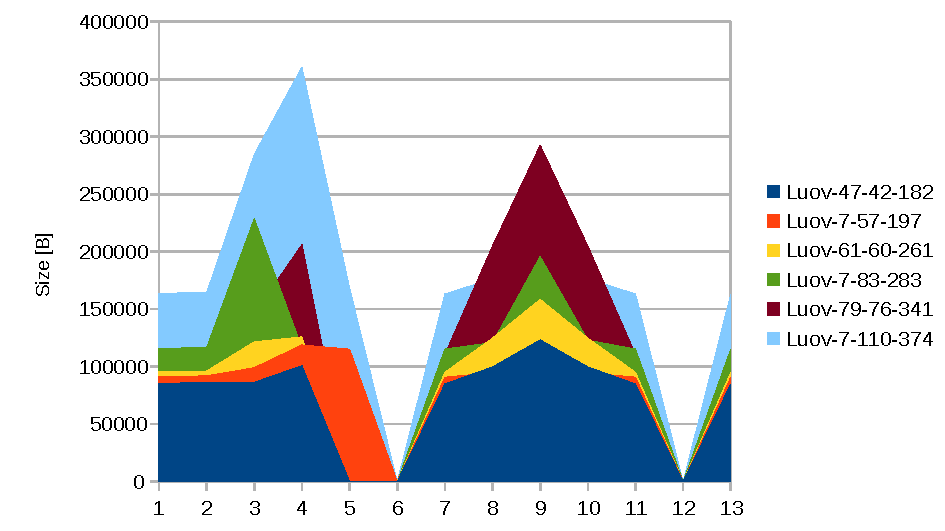
\includegraphics[width=13cm,height=7cm]{images/mem-luov0.pdf}
\caption{Memory requirement of LUOV on ESP32}
\label{mem-luov0}
\end{figure}

\bigskip\bigskip\bigskip
\begin{figure}[H]
\centering
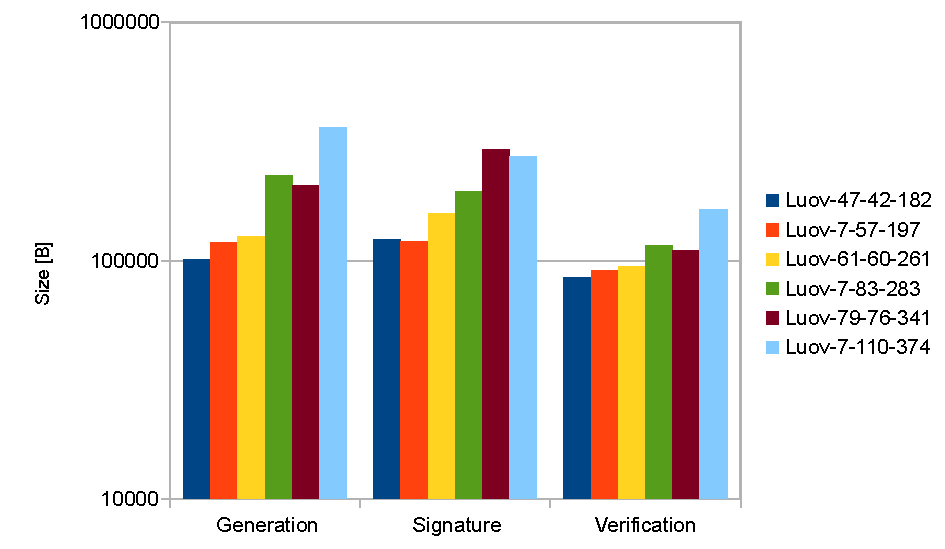
\includegraphics[width=13cm,height=7cm]{images/mem-luov.pdf}
\caption{Memory requirement of LUOV on ESP32}
\label{mem-luov}
\end{figure}

\newpage
\noindent
On the next graph \ref{mem-rb} is displayed memory allocation of Rainbow scheme. Again, there is displayed that with higher security category the implementation needs more memory but some of the Rainbow variants need suspiciously the same amount of memory, around 4MB, for example \textit{Rb-256-68-36-36-com} or \textit{Rb-256-92-48-48-com}. However, this same allocation of memory can be seen on RB variant \textit{Rb-16-32-32-32-cyc} in the verification stage. 

\begin{figure}[H]
\centering
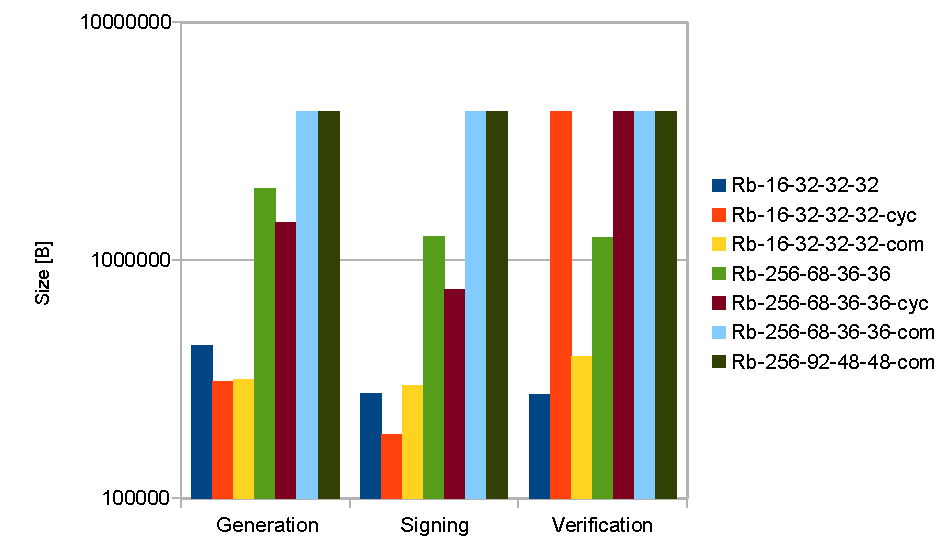
\includegraphics[width=13cm,height=7cm]{images/mem-rb.pdf}
\caption{Memory requirement of RB on ESP32}
\label{mem-rb}
\end{figure}

\noindent
I can think only of two possibilities why there is this result:
\begin{itemize}
\item	Error in measurement - In my implementation of memory measurement on ESP32 is some kind of error which input this result. But it is only few lines of C++ code which directly use the \textit{esp} API. That is why I am inclined to the second possibility.
\item	Wrong allocation - The ESP32-LyraT just allocate the rest of free memory in external RAM. This can happen when there was not enough time after free operation and the allocation table was not updated, so it used next free block. Or the segmentation of memory was not optimal and the needed memory block was not able to be allocated in previous blocks because it require bigger capacity.
\end{itemize}

\bigskip
\noindent
From these results I can assume that minimum of 4MB RAM is needed to safely run the Rainbow implementation on ESP32-LyraT. It is also visible that having public key in the form of seed save some of the memory (comparison of \textit{cyc} and classic variants).

\begin{figure}[H]
\centering
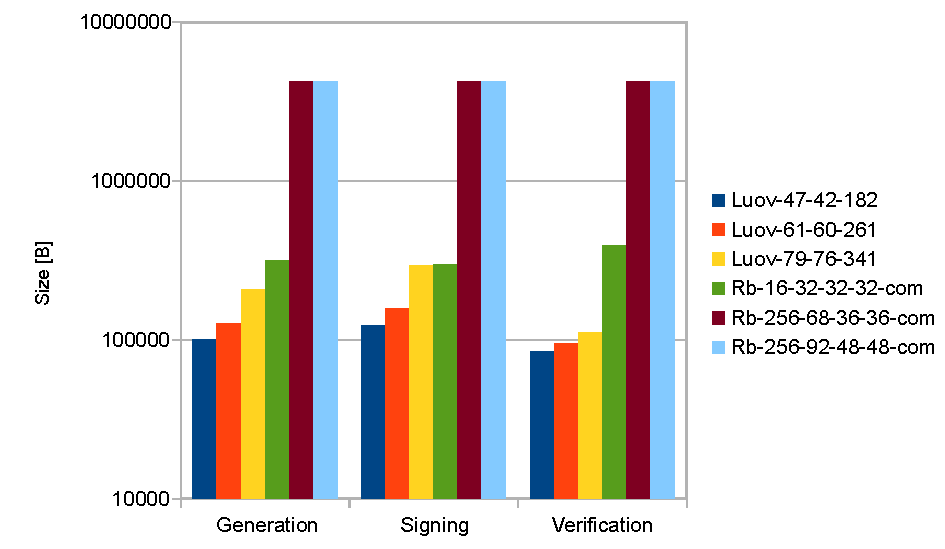
\includegraphics[width=13cm,height=7cm]{images/mem-both.pdf}
\caption{Memory requirement of implementations on ESP32}
\label{mem-both}
\end{figure}

\noindent
Graph \ref{mem-both} shows comparison of LUOV and RB schemes in memory requirements. LUOV is again better implementation in memory management. But because of this strange memory allocation in RB cases I created flag \textit{MY\_ESP\_MALLOC}, see \ref{esp-rb-memory}. With this flag I got information about every \textit{malloc} and \textit{free} in the implementation and was able to create graph \ref{mem-my-alloc}.

\begin{figure}[H]
\centering
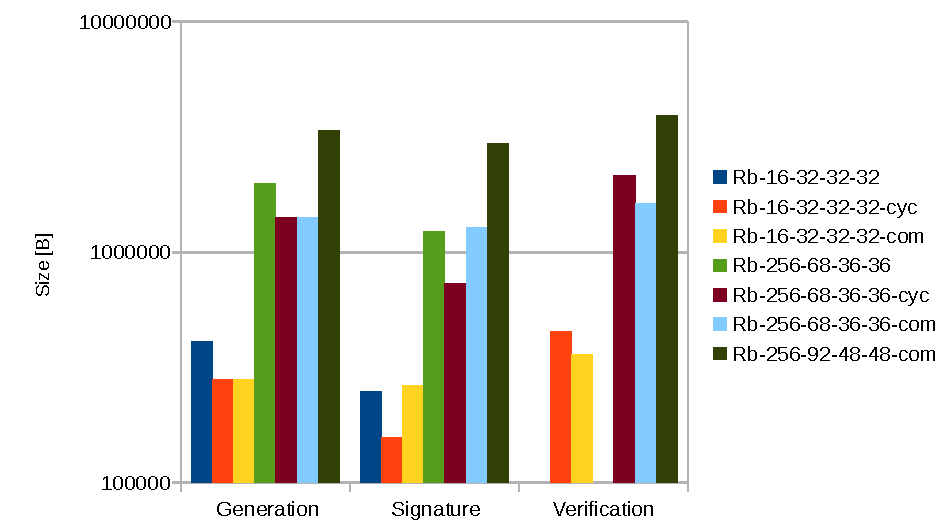
\includegraphics[width=13cm,height=7cm]{images/mem-my_esp_malloc.pdf}
\caption{Memory requirement of my\_ESP32\_malloc}
\label{mem-my-alloc}
\end{figure}

\noindent
Compared to graph \ref{mem-rb} now is possible to see more meaningful results of memory allocation but be aware that there are heap allocations of bare implementation without system libraries.

\bigskip
\noindent
On the graph \ref{mem-my-alloc} is visible that \textit{cyc} variants of RB are using the seed for public key because memory needs are lower in signature stage but high in verification stage compared to classic variants. Also is beautifully visible the use of seed for private key in \textit{com} variants. In signature stage it needs more memory then \textit{cyc} variant because of generation of private key from the seed but in verification stage it saves the memory because the private key is only in the form of small seed.

%%%%%%%%%%%%%%%%%%%
\subsection{Keys \& signature} \label{key_sign}
In this section is comparison of size of keys for different variants of signature algorithms. Must be said that the size of keys of ESP32 implementations are the same as PC implementation. I noted them from the measurement of ESP32 implementations.

\bigskip
\noindent
On the graph \ref{sign-luov} is shown LOUV sizes of public key, private (secret) key and signature. It is visible that LUOV implementation uses the same length of seed for its secret key. Also, can be seen the variants with shorter signature (\textit{Luov-7}) which can be up to 10 times shorter compared to their LUOV equivalents in NIST security category.

\bigskip
\noindent
On the other side, on the same graph is shown that with shorter signature the variants need much more space for public key which can be longer up to 3 times if I compare the \textit{Luov-7-110-374} and \textit{Luov-79-76-341}.

\bigskip
\noindent
The variants of LUOV shows kind of large difference in these two values that means it depends on the situation which of the variant will be more advantageous to use.  

\begin{figure}[H]
\centering
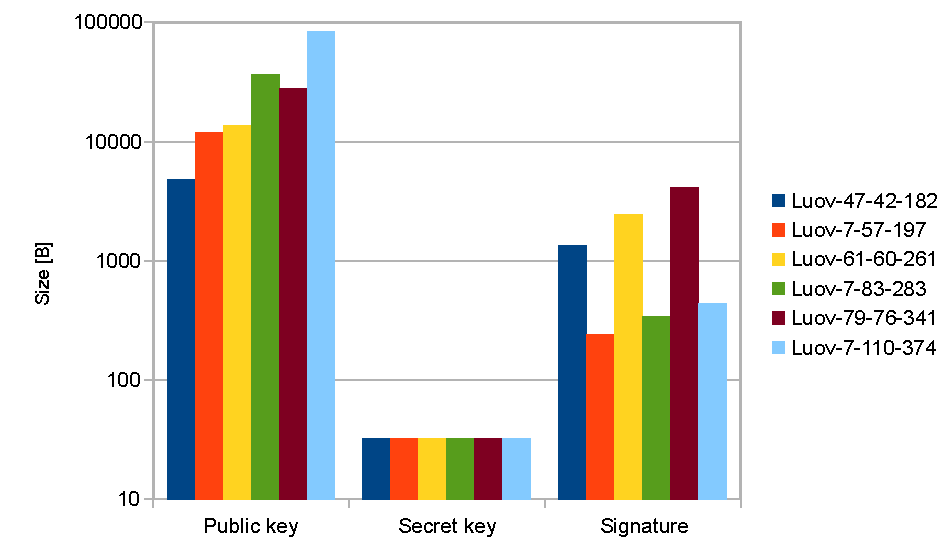
\includegraphics[width=13cm,height=7cm]{images/sign-luov.pdf}
\caption{Size of signature of LUOV on ESP32}
\label{sign-luov}
\end{figure}

\begin{figure}[H]
\centering
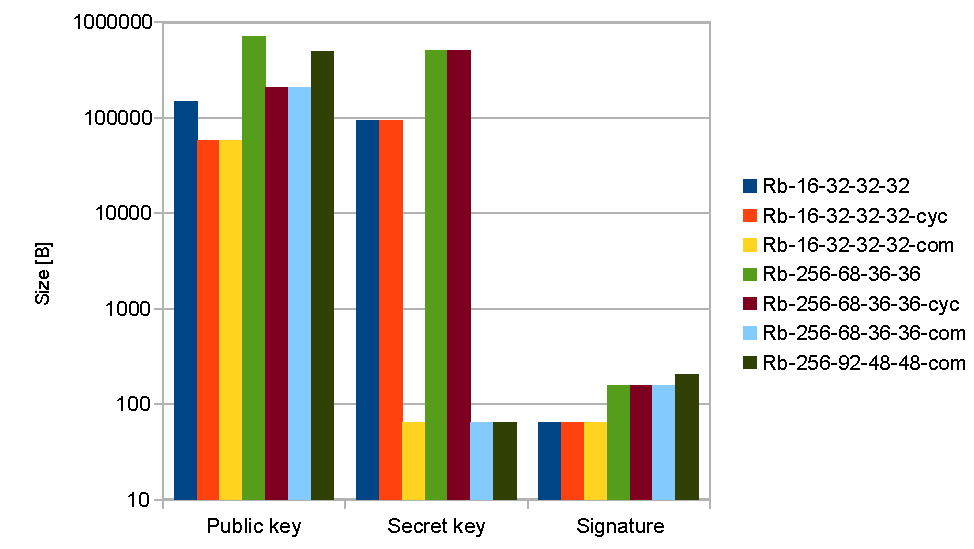
\includegraphics[width=13cm,height=7cm]{images/sign-rb.pdf}
\caption{Size of signature of RB on ESP32}
\label{sign-rb}
\end{figure}

\noindent
Graph \ref{sign-rb} displays size of keys and signature of Rainbow variants. It shows when the seed is used for secret key in \textit{com} variants it saves lot of space, the seed is only the size of 64B. For the public key in the \textit{cyc} variants the memory size was reduced by 2.5 to 3.5 times. The signature is longer (bigger) with the stronger security category but for the variant \textit{Rb-256-92-48-48-com} it is only 204B, that is an amount almost to nothing if is considered that it is spoken about NIST security category V.

\bigskip
\noindent
Next two graphs \ref{sign-all1} and \ref{sign-all2} show comparison between LOUV and RB. The first one is comparison between LUOV variants with shorter public key and RB, and the second between LOUV with shorter signature and RB. I split it into two graphs for a better comparison, especially because of the signature.

\bigskip
\noindent
On both of the graphs is shown that LOUV use shorter seed for the secret key. In numbers it is 32B for LUOV and 64B for RB. But comparison of the signatures show that RB implementation has them shorter also in both graphs. The size of RB signature is 204B, LOUV with shorter signature it is 440B and with short public key it is 4134B in security category V.

\bigskip
\noindent
The public key of LUOV is shorter in both of the graphs quite by a lot. In the first graph it is up to 17 times and in the second graph up to 6 times.

\bigskip
\noindent
From these results in this section are evident that the only benefit of Rainbow implementation is short signature which can maybe be very beneficial, for example in some congested networks.

\begin{figure}[H]
\centering
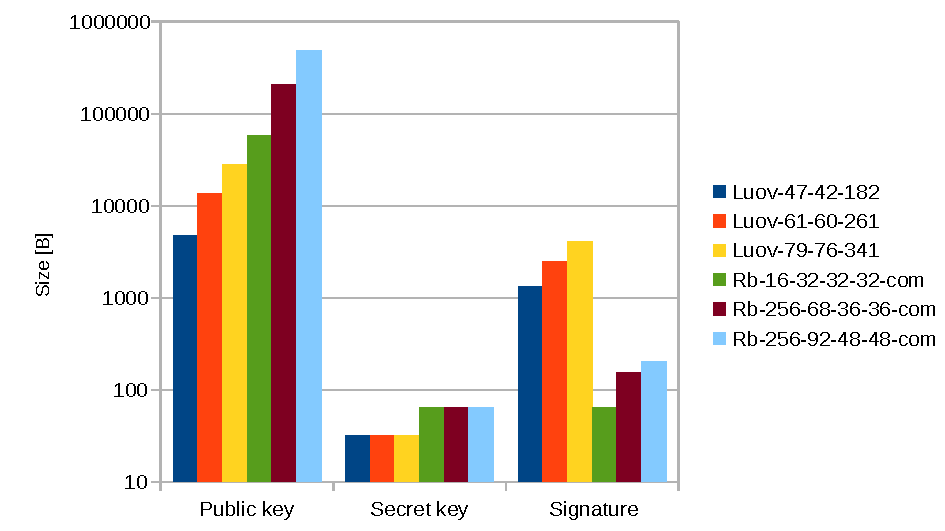
\includegraphics[width=13cm,height=7cm]{images/mem-sign-all1.pdf}
\caption{Comparison of LUOV with short public key and RB}
\label{sign-all1}
\end{figure}

\bigskip\bigskip\bigskip
\begin{figure}[H]
\centering
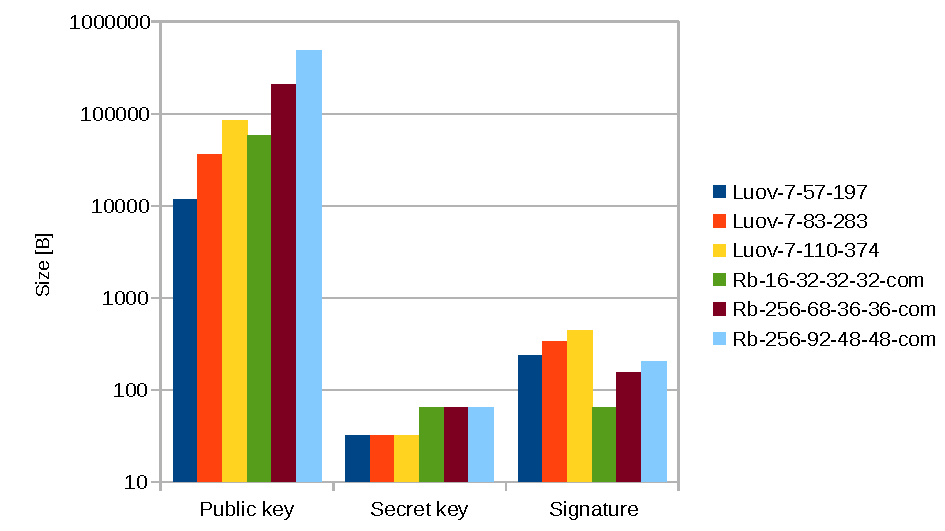
\includegraphics[width=13cm,height=7cm]{images/mem-sign-all2.pdf}
\caption{Comparison of LUOV with short signature and RB}
\label{sign-all2}
\end{figure}

%%%%%%%%%%%%%%%%%%%
\newpage
\subsection{Conclusion note}
The measured values show that the implementation of LOUV is almost better in everything compared to RB. And also, the results of time measurements of implementations on ESP32 are similar (if I do not count the general slowdown due to slower processor) to implementations on PC which should be.

\bigskip
\noindent
Rainbow has shorter signature length how can be seen on graph \ref{sign-all1} and \ref{sign-all2} but that is all. It needs much more memory for runnig (in some cases it allocates all available memory) and is slow if I compare the \textit{cyc} variants with LUOV.

\bigskip
\noindent
But the variants without generations of key from the seed are fast, even much more faster than LUOV. On the other side, if the LUOV was not using the seed for the keys it will also be faster. It would be interesting to make the comparison of these two variants but the LUOV implementation do not contains this implementation.

\bigskip
\noindent
What I want to mention is that with higher NIST security category the difference between two variants from the same category are getting bigger and bigger. The reason for this that these variants use more resources which when compared have larger difference. 

%%%%%%%%%%%%%%%%%%%%%%%%%%%%%%%%%%%%%%%%%%%%
\newpage
\section{Conventional algorithms}
One of the important criteria in usability in an embedded environment is comparison of algorithm complexity with conventional algorithms. For this comparison I selected signature scheme of RSA and ECDSA. All of them I measured on ESP32-LyraT.

\bigskip
\noindent
Below is table of variants and its NIST security category for possible comparison. \cite{L-NIST-BOOK} Variant \textit{RSA-7680} I was not able to measure because the verification of signature is failing but it is good to have it for illustration of the difference in size of public key between categories I and III and it counterparts in ECDSA.
\begin{table}[H]
\centering
\begin{tabular}{|c|c|c|}
\hline
Alg. & Category & Bit security \\ \hline
RSA-2048 & N/A & 112 \\ \hline
RSA-3072 & I & 128 \\ \hline
RSA-4096 & N/A & 140 \\ \hline
RSA-7680 & III & 192 \\ \hline
ECDSA-256 & I & 128 \\ \hline
ECDSA-384 & III & 192 \\ \hline
ECDSA-521 & V & 256 \\ \hline
\end{tabular}
\caption{NIST security categories of conventional algorithms}
\end{table}

\begin{figure}[H]
\centering
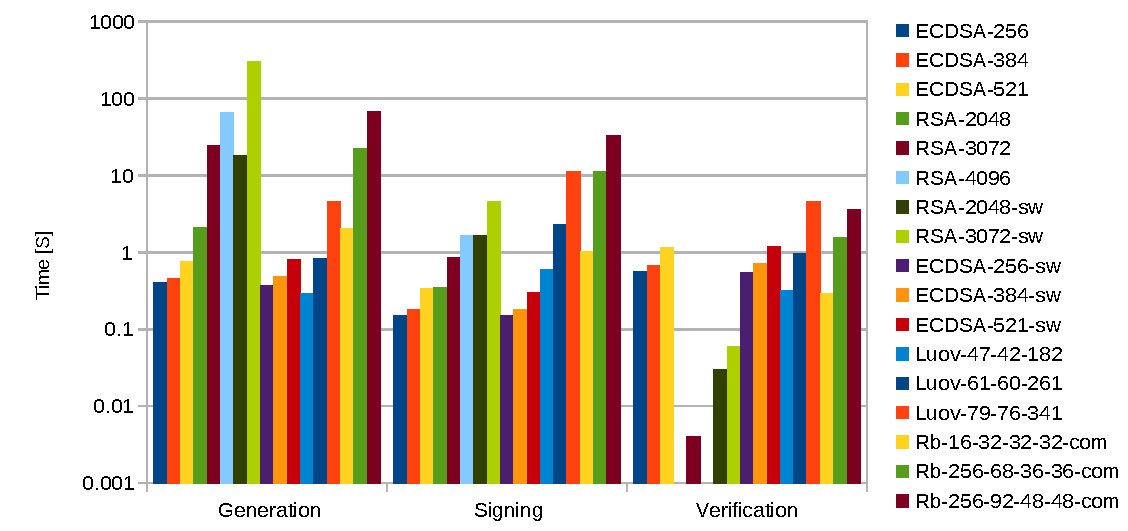
\includegraphics[width=13cm,height=7cm]{images/time-all.pdf}
\caption{Comparison with conventional algorithms}
\label{time-all}
\end{figure}

\noindent
First graph \ref{time-all} is comparison of time with algorithms selected for this thesis. It shows that ECDSA is faster than RSA except the verification. The LUOV variants shows that they are not too much slower then ECDSA, \textit{Luov-47-42-182} is even faster in generation and verification stages. If I add the difference in security category, I vs II and III vs IV, then the prospect of LUOV implementation is even better.

\bigskip
\noindent
RB variants have similar times of generation with RSA and in both cases it takes a lot of time. Also, the other stages belong to the slow side. On the other side, the variant without using the seed are really fast, faster event then the conventional algorithms. Also, the same difference in security category applies here.

\bigskip
\noindent
The ESP32 supports hardware acceleration of RSA and ECDSA. I think with this disadvantage the implementation of LUOV and RB are not lagging too much behind and can be used in embedded environment from the time point of view.

\begin{figure}[H]
\centering
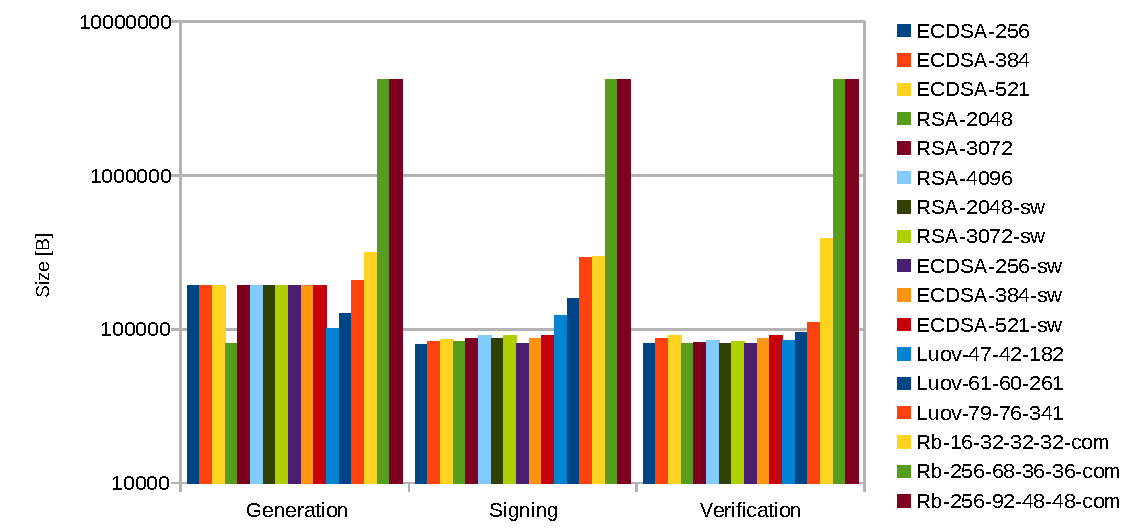
\includegraphics[width=13cm,height=7cm]{images/mem-all.pdf}
\caption{Memory requirement comparison with conventional algorithms}
\label{mem-all}
\end{figure}

\noindent
Second graph \ref{mem-all} is comparison of memory requirements with algorithms selected for this thesis. It shown that most of 
the implementations needs similar (in KB) amount of memory for its working, except the Rainbow.

\bigskip
\noindent
From this comparison it is shown that LOUV implementation is good as conventional algorithms maybe even little bit better because of the hardware acceleration and higher security category.

%%%%%%%%%%%%%%%%%%%%%%%%%%%%%%%%%%%%%%%%%%%%
%%%%%%%%%%%%%%%%%%%%%%%%%%%%%%%%%%%%%%%%%%%%
\setsecnumdepth{part}
\chapter{Conclusion}
The goal of this thesis is description of multivariate cryptography and creation of Wolfram Mathematica example for educational purpose of the selected algorithms, specifically: Unbalanced Oil \& Vintage and Rainbow. It also deals with implementation of the algorithms on PC and microcontroller, ESP32, and evaluate their memory and time complexity. Finally, it compares the implementations with conventional algorithms, RSA and ECDSA. The goal of this diploma thesis was definitely fulfilled.

\bigskip
\noindent
In the first chapter are described and defined terms used in the thesis, followed by a description of Multivariate cryptography and algorithms.

\bigskip
\noindent
The second chapter deals with the referenced implementation of algorithms, step by step examples in Wolfram Mathematica and description of ESP32 ans its implementation of algorithms.

\bigskip
\noindent
In the third and last chapter there is a description of the testing environment and the means used. It also includes measuring and testing implementations on PC and ESP32. The algorithms were then compared with each other and with other conventional signature schema implementations.

%%%%%%%%%%%%%%%%%%%%%%%%%%%%%%%%%%%%%%%%%%%%
%%%%%%%%%%%%%%%%%%%%%%%%%%%%%%%%%%%%%%%%%%%%
\bibliographystyle{iso690}
\bibliography{mybibliographyfile}

\begin{thebibliography}{9}
\bibitem{L-CZYP}
CZYPEK, P.: \textit{Implementing Multivariate Quadratic Public Key Signature Schemes on
Embedded Devices.}  Ruhr-Universit\"{a}t Bochum, 2012.

\bibitem{L-PET1}
PETZOLDT, A.: \textit{Multivariate Cryptography Part 1: Basics} [online]. 2017, [cit. 2020-04-1]. At: \url{https://2017.pqcrypto.org/school/slides/1-Basics.pdf}

\bibitem{L-PET2}
PETZOLDT, A.: \textit{Multivariate Cryptography Part 2: UOV and Rainbow} [online]. 2017, [cit. 2020-04-1]. At: \url{https://2017.pqcrypto.org/school/slides/2-UOV+Rainbow.pdf}

\bibitem{L-GEOV}
GEOVANDRO, C.C.F.P.: \textit{Introduction to Multivariate Public Key Cryptography} [online]. 2013, [cit. 2020-04-1]. At: \url{http://www.ic.unicamp.br/ascrypto2013/slides/ascrypto2013_geovandropereira.pdf}

\bibitem{L-MC0}
GOUBIN, L.; PATARIN, J.; YANG, BY.: \textit{Multivariate Cryptography.} In: van Tilborg H.C.A., Jajodia S. \textit{Encyclopedia of Cryptography and Security.} 2011, Springer, Boston, MA

\bibitem{L-MC1}
DING, J.; PETZOLDT, A.: \textit{Current State of Multivariate Cryptography.} In: \textit{IEEE Security \& Privacy.}, vol. 15, no. 4, pp. 28-36, 2017.

\bibitem{L-WIKI1}
\textit{Multivariate cryptography} [online]. 2020, [cit. 2020-04-1]. At: \url{https://en.wikipedia.org/wiki/Multivariate_cryptography}

\bibitem{L-KS98}
KIPNIS, A.; SHAMIR, A.: \textit{Cryptanalysis of the oil and vinegar signature scheme}. In \textit{CRYPTO 1998}, LNCS vol. 1462, pp. 257–266, Springer, 1998.

\bibitem{L-NIST-2ND}
\textit{NIST - Post-Quantum Cryptography, Round 2 Submissions} [online]. 2020, [cit. 2020-04-1]. At: \url{https://csrc.nist.gov/Projects/post-quantum-cryptography/round-2-submissions}

\bibitem{L-EQ-KEYS}
WOLF, CH.; PRENEEL, B.: \textit{Equivalent keys in multivariate quadratic public key systems}. In \textit{Journal of Mathematical Cryptology}, pp. 375–415, 2011.

\bibitem{L-LIFTING}
BEULLENS, W.; PRENEEL, B.: \textit{Field lifting for smaller UOV public keys}. In \textit{Progress
in Cryptology INDOCRYPT 2017: 18th International Conference on Cryptology in India}, Springer, 2017.

\bibitem{L-RB-CYC}
PETZOLDT, A.; BULYGIN, S.; BUCHMANN, J.: \textit{Multivariate
Signature Scheme with a Partially Cyclic Public Key.} In: \textit{INDOCRYPT.} 2010, vol. 6498, pp. 33 - 48. Springer, 2010.

\bibitem{L-SUB-LUOV}
CZYPEK, P.: \textit{LUOV. Signature Scheme proposal for NIST PQC Project (Round 2 version).} imec-COSIC KU Leuven, Belgium, 2019.

\bibitem{L-SUB-RB}
DING, J.: \textit{Rainbow - Algorithm Specification and Documentation. The 2nd Round Proposal.} University of Cincinnati, USA, 2019.

\bibitem{L-NIST-STANDARD}
\textit{NIST: Submission Requirements and Evaluation Criteria for the Post-Quantum Cryptography Standardization Process.} [online]. 2016, [cit. 2020-04-1]. At: \url{https://csrc.nist.gov/CSRC/media/Projects/Post-Quantum-Cryptography/documents/call-for-proposals-final-dec-2016.pdf}

\bibitem{L-NIST-BOOK}
CHANG, R.: \textit{Security-Enriched Urban Computing And Smart Grid.} 2011, Springer, Berlin

\end{thebibliography}
%%%%%%%%%%%%%%%%%%%%%%%%%%%%%%%%%%%%%%%%%%%%
%%%%%%%%%%%%%%%%%%%%%%%%%%%%%%%%%%%%%%%%%%%%
\setsecnumdepth{all}
\appendix

\chapter{Acronyms}
% \printglossaries
\begin{description}
	\item[ECDSA] Elliptic Curve Digital Signature Algorithm
	\item[IoT] Internet of Things
	\item[LUOV] Lifted Unbalanced Oil and Vinegar
	\item[MC] Multivariate cryptography
	\item[MQ] Multivariate quadratics
	\item[NIST] National Institute of Standards and Technology
	\item[OV] Oil and Vinegar
	\item[PRNG] Pseudo-random number generator
	\item[RNG] Random number generator
	\item[UOV] Unbalanced Oil and Vinegar	
\end{description}


\chapter{Contents of enclosed CD}

%change appropriately

\begin{figure}
	\dirtree{%
		.1 README.md\DTcomment{the file with CD contents description}.
		.1 exe\DTcomment{the directory with executables}.
		.1 src\DTcomment{the directory of source codes}.
		.2 esp\DTcomment{implementation for esp32 platform}.
		.2 mathematica\DTcomment{implementation in Mathematica}.
		.2 offline\DTcomment{offline reference materials}.
		.2 esp\DTcomment{implementation for PC platform}.
		.2 thesis\DTcomment{the directory of \LaTeX{} source codes of the thesis}.
		.1 text\DTcomment{the thesis text directory}.
		.2 thesis.pdf\DTcomment{the thesis text in PDF format}.
	}
\end{figure}

\end{document}
